\documentclass[10pt, a4paper]{memoir}
\usepackage{graphicx} % SO I CAN DO TWO IMAGES IN ONE PLACE HEHE
\usepackage{subcaption} % SEE ABOVE
\usepackage{hyperref} % EVERYTHING IS LINKED TO EVERYTHING ELSE ISN'T IT GREAT
\usepackage{amsmath}
\usepackage{wrapfig}
\usepackage{amssymb}
\graphicspath{ {./src/}} % LOCATION OF IMAGES

\title{Quantum Technology I, Lecture Notes}
\date{WS20/21}



% SO ANGSTROM IS NOT TAKING SO LONG TO TYPE I AM LAZY
\newcommand{\angstrom}{\textup{\AA}}

% FOR THE QUOTES
\epigraphfontsize{\small\itshape}
\setlength\epigraphwidth{10cm}
\setlength\epigraphrule{0pt}


\newenvironment{myitemize} % list then do not look so big and dumb
{ \begin{itemize}
    \setlength{\itemsep}{0pt}
    \setlength{\parskip}{0pt}
    \setlength{\parsep}{0pt}     }
{ \end{itemize}                  }


\settypeblocksize{0.8\stockheight}{0.7\stockwidth}{*}
\setlrmargins{*}{*}{1.2}
\setulmargins{*}{*}{1.4}
\checkandfixthelayout[nearest]

\begin{document}

\maketitle
\frontmatter
\tableofcontents*


\mainmatter

\chapter{Introduction}\label{ch:introduction}

This lecture script was written alongside the notes/lectures given by Professor Wunderlich in the winter semester of 20/21 at Uni Leipzig.
It is not in any way a copy of the lecture, just my interpretation.
Many phenomena he covered in the lecture I have chosen to spend more detail about, while others not.

\section{Defining Quantum Technologies}\label{sec:dqt}
The class defines it as the technology that relies on the principles of quantum physics, and how properties of quantum mechanics, like quantum entanglement, quantum superposition, quantum tunneling, etc., can breed spectacular new technologies.
An example of a few discussed in the future are listed below:
\begin{myitemize}
	\item quantum computing (also classical in some cases)
	\item quantum sensors (already commercially available)
	\item quantum cryptography (decode and encode info that can not be decoded without the knowledge of the makers)
 	\item quantum simulation (drug design)
	\item quantum metrology (connected to quantum sensors)
	\item quantum imaging
\end{myitemize}

We have come a long way since computers were first being built in the 60s.
For example, the 1969 moon lander had 2800 silicon chips and 6 transistors which correspond to 70 kilobytes (kB) of core memory, whereas the Curiosity Mars rover has a fully integrated 200 MHz chip (motherboard) corresponding to 156 MB and 2 GB RAM (keep in mind these chips on Curiosity can also resist radiation of particles on the order of $2\times 10^9$eV).
The development of these integrated circuits can be accredited to Jack Kilby of Texas Instruments, who created the first integrated circuit in 1958 (winning the Nobel Prize in 2000) consisting of a single transistor.
Today a typical Intel processor is 14 nanometers in length and has 5.6 billion transistors.
The cost of a transistor has decreased to be about $\$0.3\times 10^{-9}$.

A few of the everyday technologies brought about by quantum phenomena are listed below.
\begin{myitemize}
	\item Microelectronics (USB/Flash Memory)
	\item GPS
	\item Optical Fibers
	\item Smartphones
	\item NMR/NMI (measure spin population of hydrogen in your blood)
	\item Supercomputers
	\item WI-FI
\end{myitemize}

However, as much as we are advancing here on Earth, we still have a few hindrances.
One being Moors law, i.e., the computational power of computers is doubling every few years, but the size of chips are halving.
Currently, the IC structures are about 5 nm in size, but at some point the size of these be limited, thus the need for developing new ideas.
A neat example of quantum technology today is the USB flash memory.
The idea revolves around an NOR gate, and the use of hot electron injection for writing data and quantum tunneling for the erasure of data!

In the following chapters there will be the following content described.
\begin{myitemize}
	\item Technique (devices): accelerators, detectors, ion sources
	\item Physics: interaction of ions with matter, spin physics
	\item Ion Beam techniques: implantation, analysis
	\item Application: in semiconductor physics and in the creation of quantum mechanical systems
\end{myitemize}

Mainly we will talk about ion beams, but in order to do so, we need to know a few basic principles of ions.


\chapter{Ion Sources}\label{ch:ion-sources}

It is important to discuss ions and how they are formed such that we can accelerate them and subsequently implant them into a certain material.
The typical ion source is often a plasma ion source.
Properties of plasma like particle density, temperature, or even the geometry of confinement, play an important role on describing the particle beam we want to create.

\section{Plasma Physics Interlude}\label{sec:plasma-physics-interlude}
\epigraphfontsize{\small\itshape}
\epigraph{ A plasma is a quasi-neutral gas of charged and neutral particles which exhibit collective behaviour. }.

The particle density inside a plasma is made up of three different species: ions, electrons, and neutrals, each with their respective densities $n_i$, $n_e$, $n_n$.
An important parameter of plasma is that of charge quasi-neutrality, so the sum of all the charges should reach 0.
\[ \sum_j Q_j n_j = 0\]
It has often been said that 99\% of the matter in the universe is in the plasma state, and thus it seems we live in the 1\% of the universe in which plasmas do not occur naturally.
The reason for this can be seen from the Saha equation~\ref{eq:saha}, which tells us the amount of ionization to be expected in a gas in thermal equilibrium:

\begin{equation}
	\frac{n_i}{n_n} \approx 2.4\times 10^{15} \frac{T^{3/2}}{n_i} e^{-U_i / k_B T}
	\label{eq:saha}
\end{equation}

where $T$ is the gas temperature in Kelvin, $k_B$ is Boltzmann's constant, and $U_i$ is the ionization energy of the gas (amount of energy required to remove the outermost electron).
For ordinary air at room temperature, the fractional ionization predicted by~\ref{eq:saha} is ridiculously low: $\frac{n_i}{n_n} \approx 10^{-122}$.
One has typically in ion sources less than 10\% of atoms ionized, i.e.,
\[ \frac{n_i}{n_i + n_n} \approx \frac{n_i}{n_n} \leq 0.1 \]

The particle temperature for each of these species is normally given in eV (1 eV $\approx 11,600$ K), and although the specie temperatures may not be the same $(T_i \neq T_e)$, they can still be described by Maxwell distributions.
It is important in ion sources that the $T_i$ is as low as possible, as this will yield a 'better' beam for reasons outlined later.
\subsection{Debye Shielding}\label{subsec:debye-shielding}
A fundamental characteristic of the behaviour of a plasma is its ability to shield out electric potentials that are applied to it.
However, it is not so easy for this energy to be transferred from electron to ion, as within the plasma there is not only particle interaction, but also a phenomenon called shielding.
The interactions of the particles are due to the EM fields they produce because the particles are charged, and thus at microscopic scale, a positive charged ion will be surrounded by negatively charged electrons (shielded), and another positively charged ion further away will not be influenced that much (repulsive force is negligible) by the shielded particle ion.
This concept is quantified by a quantity called the screening distance (also called the Debye length) $\lambda_D$, and is visualized in Figure~\ref{fig:debye}.
\begin{figure}
	\centering
	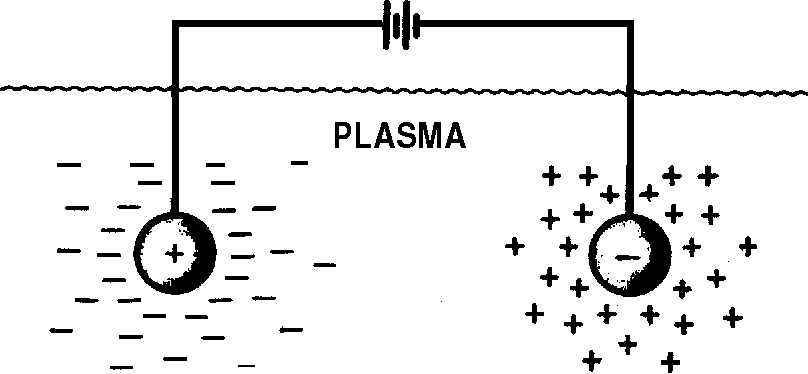
\includegraphics[scale=0.25]{debye}
	\caption{Debye Shielding of a positive charged ion in a plasma due to the collection of negatively charged electrons surrounding it~\cite{chen}.}
	\label{fig:debye}
\end{figure}
Typically the penetration of an external EM field into a plasma is given by the exponential decay $ \approx e^{-x/\lambda_D}$.
This length also describes the decay of the plasma potential $\Phi$ as it reaches a wall/boundary, meaning we must also take into account the material-plasma interface (PWI).
Typically the ions have a lower velocity than the electrons, therefore the electrons leave the plasma at a higher rate than the ions $(v_e \gg v_i)$.
This leads the plasma to be positively charged, and you will have always positively charged plasma and negatively charged walls.
The issue of charge neutrality is also a problem of plasma oscillations.
Although there is shielding, there is still interaction between ions.
One assumes in a plasma, as stated before, a quasi neutrality, i.e., if we split up the plasma into small subsections, those subsections would all be charge neutral, therefore there will be no interaction between the different regions.
The dimension of such a region is given by $\lambda_D$.

Every region described by the debye length can have some local space charges, but over the whole area the local charges cancel out leading to a charge neutrality.
If we have a dimension that is greater than the debye length, we will have charge neutrality ($x \geq \lambda_D$), and for regions smaller, we have both local and temporal fluctuations of charge ($x\leq \lambda_D$).
Within these regions smaller than the debye length, the coulomb force which pulls electrons (being much smaller in mass than the ions) resulting in an oscillatory behaviour of the particles.
Typical values of the debye length are given below:
\begin{center}
\begin{tabular} { |c |c|c|c|}
	\hline
	Plasma & $n_e (m^{-3})$ & $T_e$ & $\lambda_D$  (m) \\
	\hline
	Solar core & $10^{32}$ & $10^7$ &  $10^{-11}$ \\
	\hline
	Tokamak & $10^{20}$ & $10^8$ & $10^{-4}$ \\
	\hline
	Gas discharge & $10^{16}$ & $10^4$ & $10^{-4}$ \\
	\hline
	Interstellar Medium & $10^{4}$ & $10^4$ & $10$ \\
	\hline
\end{tabular}
\end{center}
So we are now in a position to define quasi-neutrality.
If the dimensions $L$ of a system are much larger than $\lambda_D$, then whenever local concentrations of charge arise or external potentials are introduced into the system, these are shielded out in a distance short compared to $L$, leaving the bulk of the plasma free of large electric potentials or fields.
That is, one can take $n_i \approx n_e \approx n$, where $n$ is a common density called the $\textit{plasma density}$, but not so neutral that all the interesting electromagnetic forces vanish.
Thus, the criterion for a plasma is that it be dense enough that $\lambda_D \ll L$.

\subsection{General Criterion for a Plasma}\label{subsec:general-criterion-for-a-plasma}
We have given two of three conditions of an ionized gas in order for it to be considered a plasma.
The final has to do with collisions.
By ionizing particles, we are directly influencing the particle temperature which is then related to the relaxation time(s).
An example of a relaxation time is the $90^{\circ}$ reflection time, which is the time it takes for a particle to be reflected $90^\circ$, and is not produced by a single collision, but rather a high number of small collisions summed up.
This is vastly different from the interaction of particles in gasses or solids.
Another important relaxation time is the energy relaxation time, which is the time for an energy transfer between an electron to an ion.
Plasma heating is done by externally heating electrons, and this energy needs to be transferred to the ions, so of course the time it takes for this equilibrium to be achieved is important when it comes to ion beam preparation.
Due to the different masses and densities of particles in the plasma, one must also distinguish the frequency of the oscillations of electrons and ions.
There are natural modes to these oscillations, so if we consider a single positively charged ion with a nearby electron, the electron will move much faster than the ion and overshoot the ion, and the process repeats with pulling the electron back.
This frequency of the oscillatory behaviour is described as the plasma frequency $\omega_p$, and is split into two, for the electrons $\omega_{pe}$ and for the ions $\omega_{pi}$.
\begin{gather*}
    \omega_{pe}^2 = \frac{e^2 n_e}{\epsilon_0 m_e} \approx GHZ\\
    \omega_{pi}^2 = \frac{(Ze)^2 n_i}{\epsilon_0 m_i} \approx MHz\\
\end{gather*}
Typically $\omega_{pe} > \omega_{pi}$ because of their mass difference.
If we have $\omega$ as the general frequency of the plasma, and $\tau$ is the mean time between collisions (relaxation time), we require that $\omega \tau > 1$ for the gas to behave like a plasma rather than a neutral gas.
The three conditions a plasma must satisfy are therefore:
\begin{myitemize}
	\item 1: $\lambda_D \ll L $
	\item 2: $N_D \gg 1$, where $N_D = n\frac{4}{3} \pi \lambda_D^3$, i.e., the Debye sphere
	\item 3: $\omega \tau > 1$
\end{myitemize}

\section{Ionize the particles}\label{sec:ionize-the-particles}

The question remains, how to we ionize these particles?
We know that we need to apply some amount of energy to kick the electrons away from the particles, but how much energy?
Are certain elements `better' for ionization than others? Why?
The ionization energy for different atoms varies, but follows along the periodic table, as one can see in Figure~\ref{fig:ionization_graph}.

\begin{figure}
	\centering
	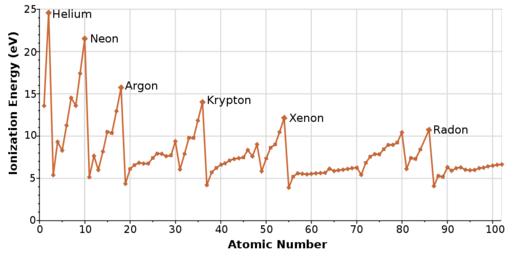
\includegraphics[width=0.8\linewidth, height=5cm]{ionization_energy_plot}
	\caption{Various ionization energies of elements.}
	\label{fig:ionization_graph}
\end{figure}


One idea to ionize atoms is through their impact via electrons.
This is possible if the energy of the electron $E_e$ is greater than or equal than the ionization potential $\Phi_i$, i.e., $E_e \geq e\Phi_i$.
Although it is possible, it is very difficult, as even then we are still working with probabilities.
For max ionization probability, we need an energy 3--4 times greater than the value of the ionization potential, so the maximum probability for ionization will decrease with higher energies.
The energy of electrons is maxwell distributed, which means that the mean energy of electrons in the plasma is given by $\langle E_e \rangle \approx \frac{3}{2} k_b T$.
If we had an ionization potential on the order of 15 eV, then we would need a very high temperature for the electrons, which normally has a range of $T_e \approx 1-10 eV$.
Due to this distribution of temperature of the electrons, it is very unlikely that we should have an electron with this temperature, and additionally this method is not very scalable.
Another idea is to use photon ionization, and this is only possible if the energy of the photon is higher than the ionization energy, $\hbar \nu \geq e\Phi_i$.
However, this is also difficult, for if we had an ionization energy of something as low as 10 eV, we would need to be using UV or x-rays to ionize the particles.
Note: This is different from laser ionized plasmas.
Aside from electron impacts within a plasma, there is also ion impacts.
This turns out to have a very low cross section and therefore not very relevant for ion sources.
It is just relevant if the speed of the ion to collide is equal to the speed of the electron on the shell of the ion, which could be on the order of 100keV. One could also use EM fields to ionize particles.
Imagine a needle with a tip that has very intense EM fields ($1.5\times 10^{10}$ V/m), which leads to an ion extraction, this is used in liquid metal sources like Gallium, or Bismuth, to wet the tip of the needle to extract the ions of these metals from the tip.
The nice aspect of the field ionization is the needle spot accuracy, being about 100 angstrom in size, leading to a great advantage in beam size having the same order of needle tip.
Besides that, one could have a beam current of up to 1 $\frac{A}{cm^2}$ which is quite nice and can be seen in Fig~\ref{fig:fib}.
\begin{figure}

	\centering
	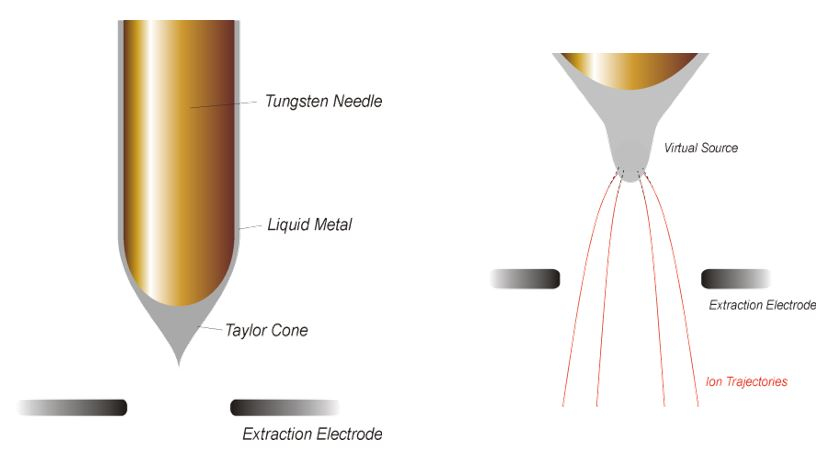
\includegraphics[width=0.8\linewidth, height=5cm]{FIB}
	\caption{During operation, gallium ions flow from a reservoir to the needle apex and a large negative voltage is applied between this needle and an extraction electrode. The balance between the electrostatic forces and the surface tension of gallium wetting the tapered W needle geometry results in the formation of a typical shape of the liquid, named Taylor cone with a half angle of 49.3°. For a typical emission current of $2\mu A$, the cone is distorted and a cusp is formed at the apex of the Taylor cone with a diameter of approximately $5 nm$. At the apex of this cusp the electric field is of the order of $1.5\times 10^{10} V/m$ sufficient to extract the ions by field emission.}
	\label{fig:fib}
\end{figure}

A main component of an ion source is something called an extractor, in which the idea is to have a confined plasma with a small aperture on one edge of it.
Near the aperture, you have a positive voltage that leads to ions to be lead out of the source, followed by a negative voltage to accelerate those extracted.
Normally with an ion beam you would use a single aperture design for a small round beam.
In order to use this beam you need a vacuum for it to travel through, with minimum pressure of $\approx 10^{-6} mbar$.
The energy of the ions extracted is given by the potential voltage of the extractor, $U_{ps}$, i.e.,  $ E_i = eZ (U_{ps} - U_{ch}) \approx eZU_{ps}$.
The reason for the dropout of the chamber voltage, is because it is normally grounded.
Due to the Debye penetration depth, and the tail speed of the electrons, the potential of the plasma is always positive, so $\Phi \approx 10V$ should also be accounted for in our equations, but the extractor voltage is normally on the order of 10 keV, so we can neglect the plasma potential.
The confinement of the plasma in the plasma source is normally done by magnetic confinement via two magnetic mirrors.
The idea is to have the increasing of a magnetic field strength at two ends of a 'bottle' causes a reflection of the ions back towards the confinement.

\subsection{Beam Parameters}\label{subsec:beam-parameters}
Once we have the ion beam generated by the ion extractor, there are a few parameters we are interested in that will determine the effects the beam.
The ion kind, if it is a gas, metal, if it is atomic or molecular in scale ($N_1^+, N_2^+$), what charge state it has $N^+, N^{++}$,  or if it is a mixture, like "Wienfilter",
the current of the ion beam, DC or pulsed ($\approx ms - ns$),
the beam energy (the energy per ion could be anywhere between eV, keV, MeV, but for example at the LHC it is TeV), which can have a magnitude between fA to mA,
the beam current, which is divided into two, the electrical current of the charges $I_e$ traveling in the beam, and the particle current $I_{par}$.
The relation of the two is: $I_e = QI_{par}$ where $Q$ is the charge state of the ion extracted (can be $Z$),
Beam shape/size is also important, as well as the beam divergence (path of beam diverges from the straight line, having an angle $\theta = 2arctan(\frac{D_f - D_i}{2l})$ where $D_i$ is the initial radius of the beam and $D_f$ is the final divergence of the beam and $l$ is the length between those two radii).


\section{Types of Ion Sources}\label{sec:types-of-ion-sources}

A sample list of ion sources is given below:
\begin{myitemize}
	\item RF ion source: one can achieve beam currents on the order of $100 \mu A$, and in principle any gas can be used.
	\item Duoplasmatron
	\item Electron Cyclotron Resonance (ECR)
	\item Single Ion Source (eg., FIB)
\end{myitemize}
All have their own benefits and are used mainly depending on which problem you wish to solve.

\section{Summary of Chapter 2}\label{sec:summary-of-chapter-2}

\begin{myitemize}
	\item Ion sources rely on plasma, and parameters of the plasma like debye shielding $\lambda_D$ play a role on the type of beam created
	\item Generating the plasma is not so simple, but can be done using either electron or photon interactions, or high EM fields (FIB)
	\item One must confine the generated plasma, traditionally done with magnetic mirrors
	\item Finally one must extract the plasma from its confinement, typically done with extractors
	\item All of these steps combine into what we call ion sources
\end{myitemize}

%! Author = adam
%! Date = 28.02.21


\chapter{Particle Accelerators}\label{ch:particle-accelerators}
So we have a source of ions, now we wish to accelerate those ions towards a sample.
There are a few main components of an accelerator, but the main concept involves using electric fields (since we have charged particles).
To ensure that these accelerated particles actually travel to a sample, we could use a closed evacuated beam-line system (a vacuum in which the particles travel) with pressure of around $10^{-5} $ mbar.
The particles need to be guided, so a deflection system consisting of an electrical beam is necessary, but also can be implemented using focussing elements like magnetic lenses.
While the ion beam is travelling, we might want to also be able to measure the beam position/current, so detectors would be nice to have in an accelerator.
Apertures, like those in a camera, could ensure a good beam quality.
Of course radiation protection equipment is necessary, but this will not be talked about so much.

There are basically two types of accelerators, and a few examples of each are given in the table below:
\begin{center}
\begin{tabular}{ c | c }
	\hline
	Electrostatic Accelerators & AC Accelerators \\
	\hline
	Van-de-Graaff / Pelletron & Cyclotron \\
	Cockcroft-Walton & Linear Acc (LINAC) \\
	& Synchrotron
\end{tabular}
\end{center}

\section{Electrostatic Accelerators}\label{sec:electrostatic-accelerators}
These were the first type of accelerators discovered and used, as they are quite simple, and much cheaper to use.
Additionally, they deliver a continuous beam, which is not possible with AC accelerators (pulsed beam), and this continuous beam then leads to a high beam current, resulting in a very 'industry friendly' accelerator.
The electrostatic accelerators can further be divided into two groups, single ended vs tandem machines.
The general design of an electrostatic accelerator is given in Figure~\ref{fig:eagen}.

\begin{figure}
	\centering
	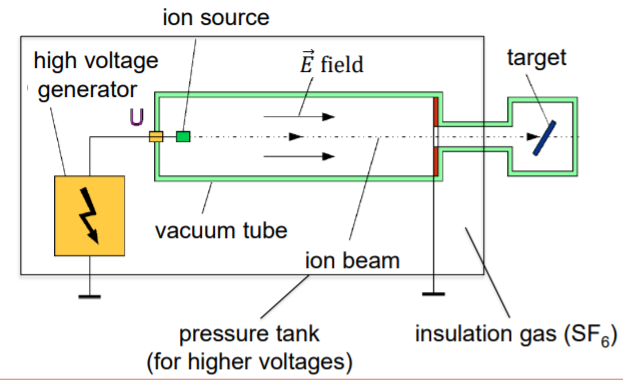
\includegraphics[width = 0.8\linewidth, height = 5cm]{general_acc_pic}
	\caption{The basic overview of ES accelerators. Surrounding the accelerator, we have a grounded insulation gas (typically SF$_6$ for its high pressure) tank, because in the vacuum chamber we will produce a very high electric field and the voltage generators will carry high voltages (several million Volts) to the ion source. The danger of breaking through the vacuum tube is high, so the insulation gas helps prevent any of these breakthroughs. The electric field moves the ions generated by the ion source.}
	\label{fig:eagen}
\end{figure}

\subsection{Single Ended Machines}\label{subsec:single-ended-machines}
\begin{wrapfigure}{r}{0.5\linewidth}
	\centering
	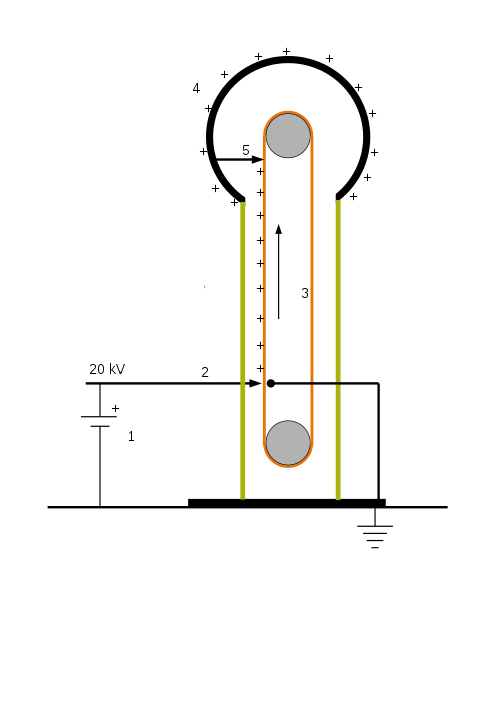
\includegraphics[scale=0.15]{degraff}
	\caption{Van-de-Graaf Generator}
	\label{fig:degraff}
\end{wrapfigure}
Incredibly high voltages are needed to produce ions for electrostatic accelerators, so we need a transformer, and one idea is to use Van-de-Graaf generators.
A 'spray' voltage brings positive charges onto an insulated charge belt (normally rubber), which transports the charges to a 'charge remover point'.
The charges are then positively charging the pressure tank, where they are able to push out the positive ion sources (same charges repel each other).
A simple equation determines the voltage in the pressure tank, $U = \frac{Q}{C}$ where $Q$ is the charges and $C$ is the capacitance of the tank apparatus.
This tank is the same as the desk experiment from high school, where you touch your hands on the big metal ball and your hair pushed up.
The first Van-de-Graff generator was 12 meters high, but with big height came with a big punch as it could generate around 5 million volts!

Nowadays, we use a similar idea, called the pelletron.
Instead of an insulating rubber band chain that carriers the positive charges, the Pelletron uses a chain with small metal segments in between.
This allows the accelerator to be charged much faster since charges are transported much faster on metal than they are on rubber bands.
For a more sophisticated approach to produce high voltages, we could use the Cockcroft-Walton high voltage cascade, which even in 1932, one could produce 700 keV protons using this method.
By alternating capacitors in a ladder like way, one is able to steadily increase the voltage, while using diodes to prevent the charges from flowing backwards.
The capacitors store up charge based on the previous capacitors plus the initial voltage.
So if we have a starting max voltage of an AC charge of 100V, and we had 4 levels of ladder, we would get a resulting voltage of 400 V.
There are no mechanical parts for this, which means less maintenance.
For each type of single ended machine discussed, the resulting energy of the ions produced is given by the equation $E_i = qU$ where $q$ is the charge of the ion, and $U$ is the potential energy of the electric field produced to accelerate the ions.

\subsection{Tandem Machines}\label{subsec:tandem-machines}

Up to now we have discussed single ended machines for accelerating ions, but now we will discuss tandem machines.
The name comes from the fact that the voltage we use to accelerate the ions is used twice.
Contrary to the single ended machine, the ion source is on ground for tandem machines.
The ions coming into the device are negatively charged, meaning that the electric field in the tank will push particles towards the center of the tank.
Then in the middle of the tank, there is what is called a 'gas stripper', and the electrons are removed from the ion, resulting in positively charged ions, which are then pushed in the same direction they were previously traveling.
A schematic is given in Figure~\ref{fig:tandem}.
The downside to this method is this gas stripper, which will 'dull' the beam, and our change in energy from the gas stripper is high.
So the beam current will not be so nice if we throw away low energy ions.
\begin{figure}
	\centering
	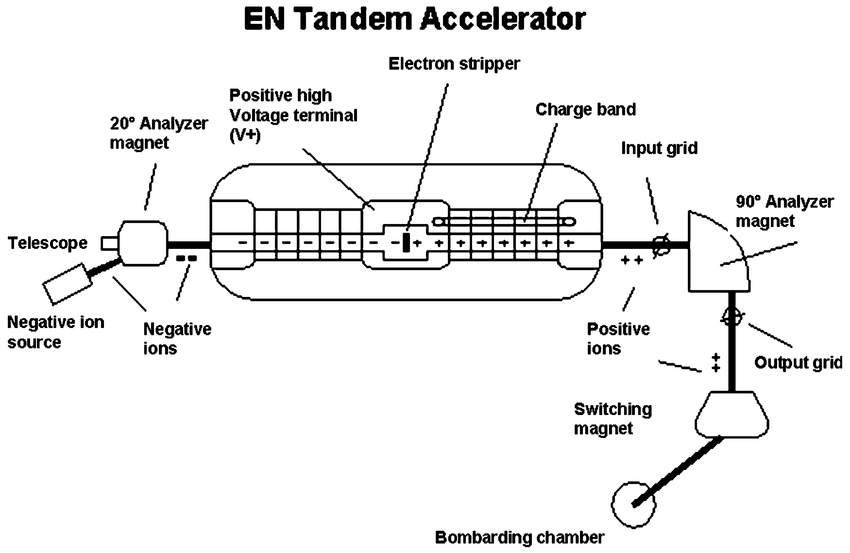
\includegraphics[width=0.8\linewidth, height=5.5cm]{Tandem-accelerator}
	\caption{The basic overview of the tandem ion accelerator. The potential is used two times. The two magnets at each end are diagnostic purposes, where we can select which ions we want to use for the ion beam. Voltages for the supply are normally around $10 MW$ resulting in 20 MeV energies. }
	\label{fig:tandem}
\end{figure}



\section{AC Accelerators}\label{sec:ac-accelerators}
AC Accelerators have an advantage over ES accelerators, which has to do with the insulation issue.
In ES systems, the insulation tanks are there to protect from catastrophe, thus limiting the voltages from becoming higher than a few mega volts.
However, AC do not have this limitation.
Also a big distinction between AC and DC accelerators is the type of ion beam produced.
For AC accelerators, we use pulsed currents (hence AC), such that the ions are not a constant flow (like in DC), but rather periodic (like a laser pulse).

\subsection{Cyclotrons}\label{subsec:cyclotrons}

There are over 2000 cyclotrons spread across the world, and have applications like the production of radio nuclide in medicine.
An examination of cyclotrons can be found in Chapter 4, section 4.1 where we discuss ion beam transport.
Applying a radio frequency range AC voltage ( $\omega = \frac{qB}{2\pi m}$) with a magnetic field perpendicular to the applied voltage, there will be a Lorentz force, guiding the particle in a circular path.
The radio frequency is set so that the particle makes one circuit during one period of this frequency $\omega$.
The velocity will increase with each path between the gaps of these 'dees'.
In the 'dees' it is a Faraday cup essentially.
On the end of one of the 'dees' there is a voltage plate used to deflect the particle into the beam line.
We can calculate using maxwell equations to find what energies are possible.
The centripetal force must be equal to the force of the magnetic field. $$ F_c = F_B \rightarrow \frac{mv^2}{r} = qvB \Rightarrow v = \frac{qBr}{m}$$
We can see that at $r \rightarrow R$ where $R$ is maximum radius of the device,\[ v = \frac{qBR}{m}\] and the maximum energy of the particle is given by
\[E_{\max} = \frac{1}{2} mv^2 \Rightarrow \frac{1}{2} \frac{(qBR)^2}{m} \]
This typically results in ion energy values of 10--500 MeV! This is much higher than the energies in electrostatic accelerators.
The problem with this is that it can be very expensive to create a large machine, and the size of the machine depends heavily on the resulting energy of the ion.
We must also take into account relativistic effects, so the frequency $\omega$ becomes $\frac{\omega_0}{\gamma} = \omega_0 \sqrt{1 - \beta^2} $, where $\beta = \frac{v}{c}$ and $\omega_0$ is the non-relativistic frequency defined above.
Because of these relativistic factor, it is not useful to use the electron, as relativistic effects occur at very low energies, whereas for high mass particles, the relativistic effects are not so apparent at useful energies.

\subsection{Betatron}\label{subsec:betatron}
In a Betatron, the changing magnetic field from the primary coil accelerates electrons injected into a vacuum torus, causing them to circle around the torus, in the same manner as current induced in the second coil of a transform.
The primary factor is a stable orbit, which satisfies the following equation:
\[\theta_0 = 2\pi r_0^2 H_0\]
where $\theta_0$ is the flux within the area enclosed by the electron orbit, $r_0$ is the radius of the electron orbit, $H_0$ is the magnetic field at $r_0$.
This means that the magnetic field at the orbit must be half the average magnetic field over its circular cross section, a condition called Wideroes condition:
\[ H_0 = \frac{1}{2}\frac{\theta_0}{\pi r_0^2} \]
This method is not used these days, but originally were used to produce electron beams up to 300 MeV.
The maximum energy is limited by the strength of the magnetic field, due to the saturation of iron and size of magnet core.
Synchrotron overcame these limitations.

\subsection{LINAC}\label{subsec:linac}
The linear accelerator starts with an ion source, followed by many 'drift tubes' in a linear connection.
Each drift tube is connected to an RF generator, so that each time an ion is between the tubes, the amplitude of the RF voltage is positive whereas in the drift tube it is negative, leading the drift tube to be a faraday cage.
The acceleration is thus between the connections of the tubes, and the length of the drift tubes need to be increased for each acceleration step.
All in all the length of each tube is based on the frequency of the driving voltage of the RF generator, as well as which particles you want to accelerate.
If we assume a constant frequency, then the period of time it takes to go through one of the drift tube, $L_n$, must be half of the frequency $f$ (particle is always accelerated in the gaps).
Wolf Widerue derived the condition for the drift tube lengths $l_n$, which is as follows: The energy of an particle being accelerated after the $n$th drift tube is given by
$$ E_n = qUn $$
where $U$ is the amplitude of the AC voltage.
This, in the classical case, is equal to
\[ E_n = \frac{m}{2}v_n^2 = \frac{m}{2} \left(\frac{l_n}{L_n}\right)^2 \rightarrow l_n = \frac{1}{f}\sqrt{\frac{nqU}{2m}} \]
The factor $L_n$ is the characteristic half period, also given by $L_n=\frac{1}{2}\frac{1}{f}$.
As we can see, with the mass being in the denominator of the equation above, for very small particles (like electrons), we need very long tube lengths if we want high energies.
It is important to note also that since we use an RF generator, we are using pulsed beams.


\section{Summary}\label{sec:summary}

\begin{myitemize}
	\item Once ions are generated we need to accelerate them, and there are two main methods to this: AC and Electrostatic
	\item Electrostatic is the cheapest and most industry friendly, and is divided into two methods, single ended vs tandem
	\item tandem machines rely on negatively charged ions, and result in high energies but not so good beam current
	\item single ended machines are generally good, can be done without the use of mechanical parts via the Cockcraft-Walton cascade
	\item AC accelerators produce ion energies much greater than the ES approach (10-100 MeV)
\end{myitemize}


%! Author = adam
%! Date = 28.02.21

\chapter{Ion Beam Transport and Optics}\label{ch:ion-beam-transport-and-optics}

Once we have accelerated the ions, we want to put them on a path towards a sample (or whatever goal you have in mind with these ions).
The path that they take cane be straight or curved, but regardless the motion is directed a combination of deflectors and lenses.
With the help of EM fields, we can not only focus particles (as is the case with normal lenses), but also accelerate or decelerate particles, as well as direct the particles onto particular paths.
This topic was introduced by Hans Bush in 1926.

\section{Deflection}\label{sec:deflection}
Deflection, as the name suggests, has to do with the directing of the particles as opposed to the accelerating or focusing of particles.
The two types of deflectors we discuss are the electrostatic and electromagnetic deflectors.
For electrostatic deflectors, we refer to those attached to the cyclotron, but the cases made generally hold for other accelerators.
The general idea involves using the Lorentz force, given below. $$ \vec{F} = q(\vec{E} + \vec{v} \times \vec{B}) $$

\subsection{Electrostatic}\label{subsec:electrostatic}

There are two general classes of electrostatic deflectors: devices on which the applied voltage is DC (Direct Current) only, and devices on which the deflecting potential is a sum of instantaneous RF (Radio Frequency) voltage on the dee and the constant DC voltage applied.
Figures of both are given in~\ref{fig:deflectors}.
Before we go into detail about the two, we first consider a simple example.
Consider two plates of opposite charge with an electric field between them.
A positively charged particle entering the area between the plates with motion parallel to the surface of the plates will then experience a pull in the direction of the field (opposite for negatively charged particles), and be deflected with a parabolic path.
The motion of the particle is no longer parallel to the surface of the plates but is then curved.
If the path was in the direction of the field lines (perpendicular to the surface of the plates), then the positively charged particle would experience an acceleration, and for a corresponding deceleration on the path in the direction opposite of the field lines.

\begin{figure}
\begin{subfigure}{0.5\textwidth}
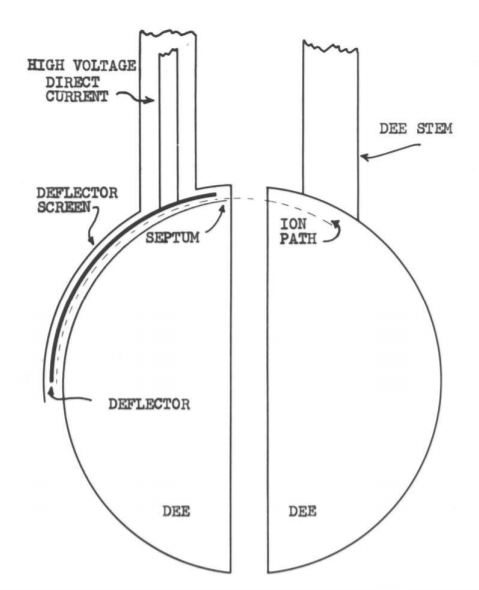
\includegraphics[width=0.9\linewidth, height=5cm]{DCdeflect.png}
\caption{A DC deflector}
\label{fig:DCdeflector}
\end{subfigure}
\begin{subfigure}{0.5\textwidth}
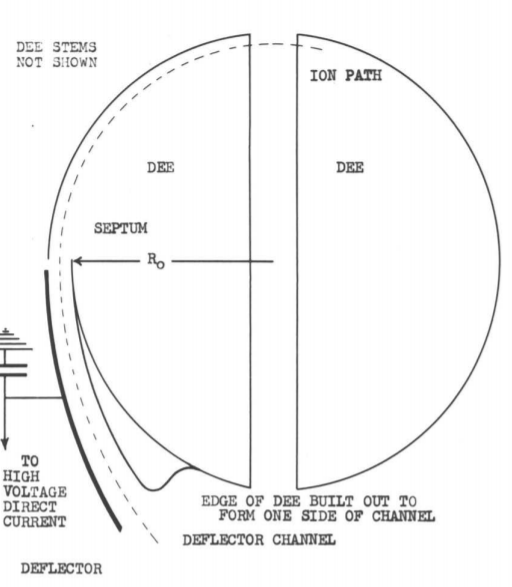
\includegraphics[width=0.9\linewidth, height=5cm]{RFdeflect.png}
\caption{A RF deflector}
\label{fig:RFdeflector}
\end{subfigure}
\caption{Two types of electrostatic deflectors, taken from~\cite{1}}
\label{fig:deflectors}
\end{figure}
The DC deflector, found in Figure~\ref{fig:DCdeflector}, allows complete control over the deflecting potential that is independent of the phase of the circulating ions.
No capacitance is added to the dee system by the deflector.
This is importance since all the power input to the dees will not be lost through the deflector.
The disadvantages of a DC deflector include the fact that incredibly high potentials are required to pull the ions away from the magnetic field which holds them in a circular path (in the case of cyclotrons, but can also be thought of generally).
If one was using an accelerator that is a low voltage (cyclotron, LINAC) then one still would need some shielding gas for the high potential of the DC deflector.
Also, any adjustment of the deflector would be a mechanical one, thus be internal and quite difficult to adjust.
These problems are eliminated by the RF deflector, seen in Figure~\ref{fig:RFdeflector}.
The RF deflector utilizes the high RF potentials existing in the cyclotron, and contains of a strip of metal extending over an arc of 60--90 degrees that forms one side of a deflecting channel.
The channel is the region through which the ions pass and in which the electrostatic field is formed.
What is called the septum is the entrance to the channel, which is a strip of metal that can be quickly tuned via a potential applied to the metal such that the deflector spacing is varied.
This is the important advantage to the RF deflector.

A simpler case is a device called the \textit{steerer}, which consists of a series connection of devices consisting of two charged plates (as discussed in the general case).
The devices are then producing electric field opposite relative to each other such that they take turns deflecting the ions such that an overall change in the particle path.
Depending on the distance between the connection of the two devices, called the drift length $d$, the ion will be deflected by a distance $\Delta a$ compared to the incident.
The end path is still parallel to the initial ion beam.
\subsection{Electromagnetic}\label{subsec:electromagnetic}

In the electromagnetic case, consider a field line similar to our example for the electrostatic case (instead of an E field, we have a B field perpendicular to the 'surface' of two plates).
For ions moving transverse to the field, it will end up in a circular path from the Lorentz force.
If the ion has a velocity component that is not perfectly perpendicular to the magnetic field, it will spiral upwards or downwards in addition to the circular motion.
For high energy particles (high velocity), it is better to use the electromagnetic deflection, as the $\vec{v}$ component of the Lorentz force dominates, and will have a bigger impact on the deflection force on the particle.
There is also what is called the magnetic field steerer as discussed in the electrostatic case.
A device consisting of a 2 magnetic dipole  in the x and y directions.
The ion is then passing through similarly, but this time we have a magnetic field is reversed from transitioning from one device to the next.
The ion is the similarly deflected, but instead of the field line being in the direction of motion in the electrostatic case, it is perpendicular (in this case if the particle is traveling left to right along the surface of this page, the first magnetic field device would produce a $\vec{B}$ field into the page, that would deflect the particle in the downward direction (relative to the writing of this page).
Then the second device would have a magnetic field directed out of the page such that the net effect of both would be a translation of the beam path as before.

\section{Lenses}\label{sec:lenses}
Now lets say we want to focus our ion beams.
Simplest case is a \textit{tube lens}.
This is similar to the combination of a convex and a concave lens in optics.
Not only does deflection occur in this lens, since a voltage is applied across the two tubes, you are also increasing the energy of the ions, since $\Delta \Phi \neq 0$, but rather $ = U$, the voltage applied.
Due to the curvature of the tubes,  similar to the shape of the convex lens, the beam is focused.
A more sophisticated design is the so called \textit{einzel lens} which can be found in Figure \ref{fig:einzel}.
Similar to the tube lens, we are using a combination of three separate tubes (cylindrical or not, just symmetric), where the middle of the three acts as the einzel lens.
This is a charged particle electrostatic lens that focuses without changing the energy of the beam.
The electrostatic potential in the lens is symmetric, so the ions will regain their initial energy on exiting the lens, although the velocity of the outer particles will be altered such that they converge on to the axis.
This causes the outer particles to arrive at the focus intersection slightly later than the ones that travel along a straight path, as they have to travel an extra distance.
The math is as follows:
The equation for the change in radial velocity for a particle if it passes between any pair of cylinders in the lens is $$\Delta v_r = \int \frac{q\vec{E}_r(\vec{r},z)}{mv_z}dz, $$ with $\textbf{z}$ axis passing through the middle of the lens and $r$ being the direction normal to $\textbf{z}$.
If the lens is constructed with cylindrical electrodes, the field is symmetrical around $\textbf{z}$.
The magnitude of the electric field in the radial direction for a particle at a particular radial distance and distance across the gap, is given by $\vec{E}_r(\vec{r},z)$, and $m$ is the mass of the particle passing through the field.
$v_z$ is the velocity of the particle and $q$ the charge.
The integral occurs over the gap between the plates, where the lensing occurs.

\begin{figure}
	\centering
	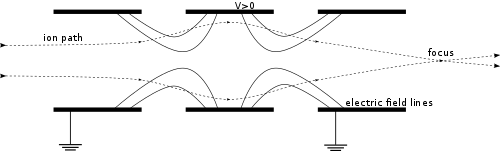
\includegraphics[width=0.9\linewidth, height=5cm]{Einzel_lens_draw.svg.png}
	\caption{Einzel lens configuration. It is important to note that ions traveling near the top or bottom (closer to the cylinders) will have a longer path than those in the middle of the cylinders. This will result in ions being seperated in time, since they are all traveling the same velocity (assuming they had the same initial velocities) as the einzel lens does not accelerate the ions. }
	\label{fig:einzel}
\end{figure}

Another interesting lens is the quadrupole lens.
These are often used in ion trapping, but can also be used in the lens cases.
The mathematics works the same as if you were to use multipole lens, where we include transfer matrices and such.
The general equation for a magnetic field is a combination of terms corresponding to the type of pole you are using.
For example, assume you have a particle traveling in the $z$ direction, and regardless of how many poles you use, your magnetic field is in the $x$ and $y$ directions, i.e., $\vec{v}= (0, 0, v_s)$, $\vec{B} = (B_x, B_y, 0)$.
Then the force acting on the particle is $F = mv_s^2 / R$ where $R$ is the radius of the circular motion of the particle.
We can split up the components of the force in the $x$ direction, perpendicular to the velocity of the particle as $F_x = -qv_sB_y$, and the radius of the motion is given by $1/R(x,y,z) = \frac{q}{p}B_y(x,y,s)$. This term on the RHS dependent on the type of pole you use. So the combination would be:
$$ \frac{q}{p}B_y(x) = \frac{q}{p}\left( B_y(0) + \frac{\partial B_y}{\partial x} x + \frac{1}{2!}\frac{\partial^2 B_y}{\partial x^2} x^2 + \frac{1}{3!}\frac{\partial^3 B_y}{\partial x^3} x^3 + \dots\right) $$  The first term on the RHS is the dipol and the second the quadrapol. These two are called terms of linear ion optics, whereas the next two, the sextupol and oktopul, correspond to non-linear ion optics.
Lens configurations can get as complicated as one wishes, for example the omega lens, or bessel box photon stop.
In order to verify if a lens system will work before the money is spent in building it, it is often recommend to simulate your structure before hand.
Simulation software like \href{https://simion.com/}{SIMION} work well in this.

\section{Selectors}
Let's say you did a handful of focusing lenses and deflectors, and now you have a wide variety of ions with different energies.
You may want to select ions with a particular energy.
In that case you can use what are called velocity selectors.
These can be as complicated as quadrupole magnets, or as simple as a Wien filter.
Basically you introduce a magnetic field and or electric field such that the particles that which have the appropriate (desired) velocity (for Wien filter: $v = \frac{E}{B}$), are passed through the 'filter'.
Those that do not drop off in contact with the filter.

\section{Summary}

\begin{myitemize}
	\item Once a particle is sufficiently accelerated, we can use lens/deflectors to control the beam to a destination using only the Lorentz force
	\item Deflectors can be as simple as a combination of charged plates that translate the ion beam path a distance away from the original path, these devices are called steerers
	\item Lens work similarly to optical lenses, but by using EM fields, examples include the tube lens as well as the einzel lens.
	\item Lenses can not only focus but also accelerate particles.
	\item Electrostatic and Magnetic lenses can also be used to select particles of a certain energy.
    Monochromatic beams can be created using this method of velocity selection (see Wien Filter).
\end{myitemize}
%! Author = adam
%! Date = 28.02.21


\chapter{Beam Parameters}\label{ch:beam-parameters}

Once we have a focused beam of ions hurtling themselves at high energies towards a sample, there are a few parameters that are of particular use in both the description of the beam, and the predicting of effects of the beam.
Below is a list of parameters, and those that we will cover in closer detail are listed in \textbf{bold}.
\begin{myitemize}
	\item DC or AC
	\item Ion Type
	\item Ion Energy
	\item Charge State
	\item \textbf{Divergence, Brightness (Brilliance), Emittance}
	\item Beam Diameter
	\item \textbf{Focus Size}
	\item Working Distance
	\item \textbf{Beam Current }
	\item \textbf{Beam Shape}
	\item Beam Stability
\end{myitemize}
For example, AC or DC is a question we have already discussed in CHAPTER ION ACCELERATORS, in which beams could be a constant supply (DC), or are pulsed (AC).
In the chapter on ion sources we discussed how one would produce different ions, hence the ion types.
Ion energy is also discussed in \ref{ch:ion-sources}, but it also depends on the charge state of the ion.
The lowest beam diameter we can achieve is known as the focus size.
The beam current being the density of ions traveling towards a sample, which one may want high or low current depending on application, e.g., you want to introduce single ions into a sample, so you want very low current so that a singular ion impact is possible.

\section{Emittance and Brilliance}
In order to best understand these concepts we must revisit our lectures on theoretical mechanics, and more specifically \textit{Liouville's Theorem} and phase space.
The goal is to describe the trajectory of particles using phase space.
Liouville's Theorem helps in this regard with the fact that a volume in phase space is constant in time iff one can describe their system using a Hamiltonian.
In ion beams we normally have phase ellipse, i.e., the phase space of the ion beam is roughly in the shape of an ellipse.
The equation for a 2D ellipse is given by\[ \gamma x^2 + 2\alpha x x^{\prime} + \beta x^{\prime 2} = \epsilon \], for which the area of this 2D ellipse is given by: \[ \int_{ellipse} dxdx^\prime = \pi \epsilon \].
In both of these equations, we are in phase space, so $x$ is the position, and $x^\prime$ would be the momentum.
The phase space distribution function would then be constant along the trajectories of the system (in our case this is the ion particle system), which leads to the density of system points in vicinity of a given system point traveling through phase space is constant with time.
In the Figure~\ref{fig:PSib} we see how the phase space is changing due to a focusing lens.
But what does the brightness and emittance have to do with all of this?

\begin{figure}
	\centering
	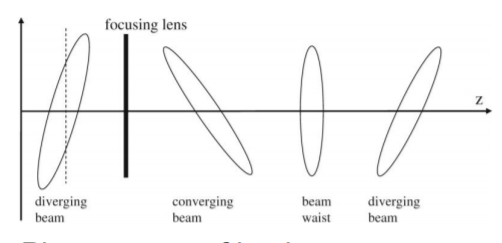
\includegraphics[width=0.7\linewidth, height = 5.5cm]{phase-space-lens}
	\caption{Via the use of a focusing lens, we see that the phase space of the diverging beam is inverted to that of the phase space of the converging beam. Then, as we reach the focal point of the beam from the use of the lens, we see that the distribution of ions has a very small width, i.e., they are centered positionally in the phase space (the focus) and the position unceratnity is low whereas there is broad uncertanity in the momentum! After the beam waist, we see the beam transforms back into a diverging beam, and we a similar phase space as we got before.  }
	\label{fig:PSib}
\end{figure}
Emittance is the measure for the average spread of particle coordinates in te phase space.
Since we clarified that the volume (or area in 2D) of the phase space stays the same over time through accelerations (lens, etc.) the position spread may change, but the emittance stays the same.
A low emittance particle beam is a beam where the particles are confined to a small distance but have nearly the same momentum.
This goes to say that a beam system will only allow particles with a particular momentum, and of course those that fit through the beam pip or magnets that make up the system.
For the geometric definition, one will see why we chose $\epsilon$ above in our definitions.
The  definition of the transverse emittance $\epsilon$ is:
\[ \epsilon = \frac{6\pi \left(width^2 - D^2 \left(\frac{dp}{p}\right)^2\right)}{B}\]
where $width$ is the width of the particle beam, $dp/p$ is the momentum spread of the beam, $D$ is the value of the dispersion function at a measurement point in the particle accelerator, $B$ is the value of the beta function at the same measurement point.
Emittance also closely related to the brightness of a beam, and can be seen in Figure~\ref{fig:bright}, where we derive equation~\ref{eq:bright}.

\begin{figure}
	\centering
	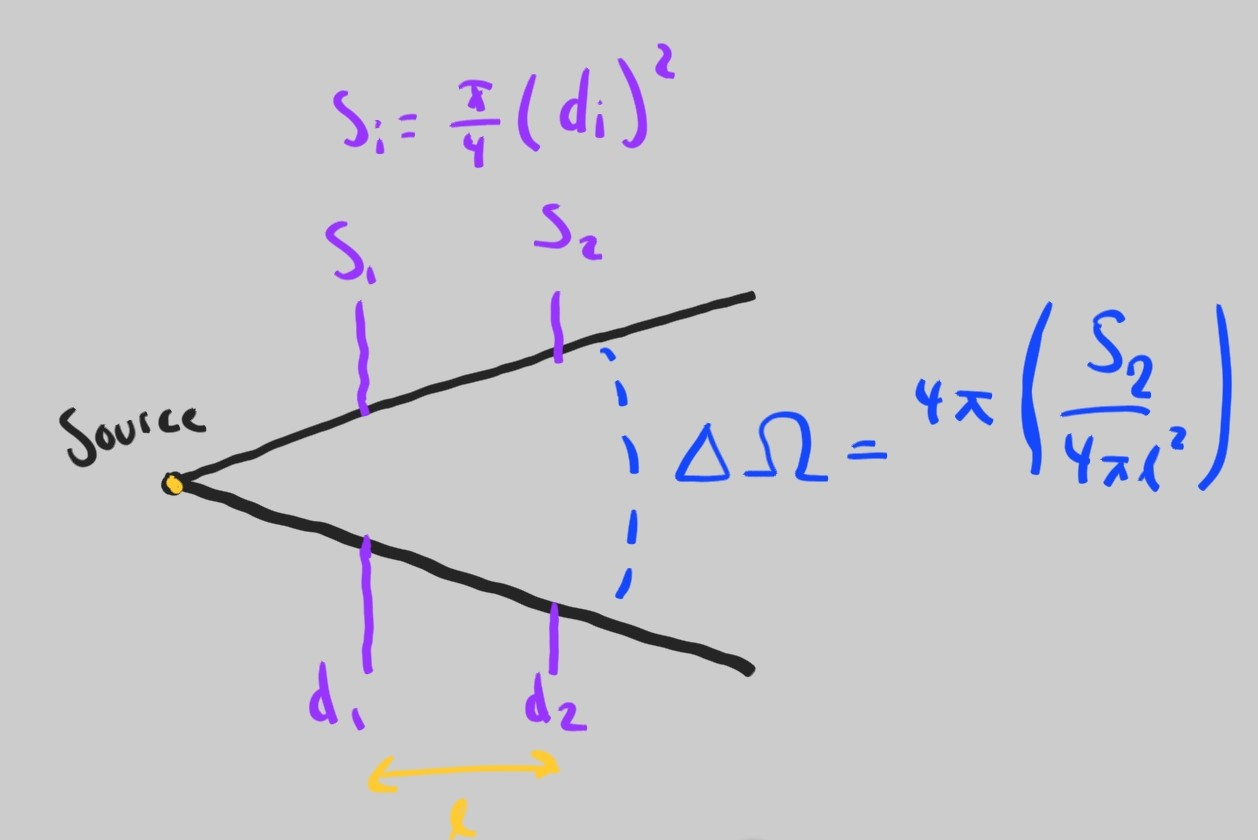
\includegraphics[width=0.5\linewidth, height=5cm]{bright}
	\caption{The ion source on the left hand side passes through two apertures $A1$ and $A2$, each aperture having a diameter denoted by $d_1$, $d_2$ and are placed a distance $l$ apart from each other. The area of the apertures is then written $S_i = \frac{\pi}{4}d_i^2$. The divergence of the beam is denoted by the solid angle $\Delta \Omega$. At the end of the second aperture we want to measure the beam current, so we place a Faraday cup grounded (the apertures are also grounded). Now the brightness is then defined $B = \frac{I}{S_1 \Delta \Omega}$. The solid angle is $\Delta \Omega = 4\pi \frac{S_2}{O}$ where  $O$ is the overall solid angle, i.e., $4\pi l^2$. This yields us finally the relationship seen in Equation \ref{eq:bright}}
	\label{fig:bright}
\end{figure}


\begin{equation}
B = \frac{I l^2}{S_1 S_2}
\label{eq:bright}
\end{equation}

There is also an equation where we normalize the brilliance w.r.t the energy of the ions $E$, which can be written:
$$ B_n = \frac{I l^2}{S_1 S_2 E} $$
For example, an ion beam with current $1.1$nA, and aperture lengths $d_1 = d_2 = 2-- \mu$m, and distance $l = 4.9$m between them, the normalize brilliance of the ion beam for ion energy $E = 2 MeV$ is $B_n = 13.5$ A/m$^2$eV.


Although emittance is normally constant, there are times when it is not.
Lens, for example, conserve it but when we use radiation damping or electron cooling, there are other effects taking place on the ions such that there can be changes in $\epsilon$


\section{Focus Size}\label{sec:focus-size}
As mentioned earlier in the chapter, the focus size is defined as the lowest possible beam diameter one can achieve.
One can focus a beam using magnetic lens just like how optical focusing works.

\section{Beam Shape}\label{sec:beam-shape}
The size of the beam is influenced by geometric demagnetization of the lens system, as well as aberration of lenses and the beam emittance.
There are many fancy ways in measuring the beam profile.
Another aspect of the beam profile is the temperature of it.
Like a collection of gas molecules, the ion beam also has a temperature.
Since particles will naturally drift apart in the accelerator (think expanding gas particles of a particular temperature), the beams must be then brought back together or else they will slam into the walls of the vacuum pipes.
But, because of this, one must think about how the ion-ion interaction is.
Let's estimate the Coulomb force between two ions.
We can estimate using a ion beam current of $I = 1$ MeV, which gives us avelocity of about 10 precent the speed of light, or $v = 3\times 10^7 $m/s.
With this current we have a number density per second of $I = \frac{Q}{t} = \frac{Ne}{t} \Rightarrow n = \frac{N}{t} \approx 6.2\times 10^5$ ions per second.
The distance per ion is then estimated $  \frac{v}{n} \approx 4.8$ mm per ion.
This finally yields us $F_C \approx 10^-23$N.
Okay it is tiny.
The Coulomb interaction can be neglected for this example, but as we said earlier, at high density, the Coulomb interaction will be much larger since the distance between ions will be much smaller!


\section{Summary}\label{sec:summary2}

\begin{itemize}
	\item Many parameters of an ion beam can be quantified, and many come from the source/acceleration.
	\item The emittance of an ion beam $\epsilon$ is held constant through the use of lenses/acceleration of particles, but can also at times not be constant due to non-linear affects (high $I \rightarrow$ high $n$ thus interactions can not be neglected) as well as radiation damping, etc.
	\item Brilliance of a beam measures the current density over an area in which the beam is focused
	\item Focus size is the lowest possible beam diameter one can achieve
	\item Beam shape is influenced by the aberration of lenses and beam emittance
	\item With low current density we can neglect the ion-ion interaction, but at higher densities we must take this into account
	\item  The measuring of a current is through the use of a faraday cup
\end{itemize}


%! Author = adam
%! Date = 28.02.21

\chapter{Basics of Interactions of Ions with Matter}\label{ch:basics-of-interactions-of-ions-with-matter}
Well to put together what we have done so far: Ion Sources $\rightarrow$ accelerating those ions $\rightarrow$ transporting those ions $\rightarrow$ quantifying the important parameters of your final ion beam.

I'd say we are ready to start having these ions interact with matter!
Some keywords before we begin:

\begin{myitemize}
\item Ion penetration depth
\item sputtering
\item doping with foreign atoms
\item change of mechanical, optical, electrical, and magnetic properties
\end{myitemize}

\section{Interaction Forces in Solids and Vacuums}\label{sec:interaction-forces-in-solids-and-vaccums}
When we want to discuss how ions interact with matter, we must examine in detail the short and long range inter-atomic forces.
For the simple case, in a vacuum, we have two extrema of interaction for two particles with charges $Z_1$ and $Z_2$.
At the long range interaction, we have the Coulomb electrostatic interaction, which has a potential:
$$V_c(\vec{r}) = -\frac{Z_1 Z_2 e^2}{\vec{r}}$$
where $\vec{r}$ is the distance vector between the two.
This scales with $\propto \frac{1}{r}$, but it is important to note that this long range interaction potential exists only when both particles are charged!
On the other side, the short range interaction, we have quantum mechanic forces governing, for example the Pauli exclusion principle.
This regime in which short range applies is when atomic orbital overlap.
This interaction exists even when particles are neutral, which is not the case for the long range interaction, so these short range interactions can happen for ion-atom or atom-atom combinations.
If we turn our attention outside a vacuum, and into a solid, we have the Lennard-Jones potential as seen in Figure~\ref{fig:LJPfig}.
The reason we use this is that the voltage in a solid or crystal is normally unknown, or at least very complex, so the LJP is a nice approximation.
This potential depends on the interaction distance $\vec{r}$ and is given by:
$$V(\vec{r}) = \frac{pq}{p-q} \Delta E \left[ \frac{1}{p} \left( \frac{r_0}{r} \right)^p - \frac{1}{q} \left( \frac{r_0}{r}\right)^q \right]  $$
In this rendition of the LJP, $p$ and $q$ are fitting parameters, but the important part of this equation is $\Delta E$ which is the energy at the equilibrium atomic distance $r_0$, i.e., $\Delta E = V(r_0)$.
It can also be considered the binding energy of the atom into the solid, i.e., the energy one must apply to pull out the atom from the crystal into the free space.
If the atom is in the inter-atomic distance $r_0$, then it is in the most stable configuration of the atom in the solid.
In reality, the potential will probably look something different from that of the LJP, but it is a good model and easy to handle.
\begin{figure}
	\centering
	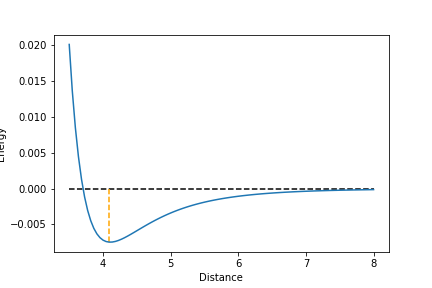
\includegraphics[width=0.6\linewidth, height=6cm]{LJP}
	\caption{The orange dashed line represents $\Delta E$, i.e., the energy at the equilibrium atomic distance $r_0$. }
	\label{fig:LJPfig}
\end{figure}

\section{Collisions of Ions with Atoms}\label{sec:collisions-of-ions-with-atoms}
Now we imagine an ion with energy $E$ flying towards a target atom.
Depending on the energy of the ion, there will be different minimum interacting distances $r$ during the scattering process.
At impact, the wave functions of the ion and atom will overlap, so it is very important to know the inter-atomic potential of the sample.
If we have a high $E$, then we have a low $r$, and with low energy ion $E$, then there will be a high $r$.
However, this is a many body problem, so we will have nuclei and electrons of the ions as well as those in the atoms factoring into the potential, which in turn will be very complex, since we must take into account the interaction of electrons and nuclei.
So we must consider realistically two reference points: the Bohr radius $a_0 = 0.5\angstrom$ and $r_0$ from the LJP (the spacing of atoms in a crystal).
If $r >> r_0$, the crystal atoms are undisturbed by the incoming ion.
When $r << a_0$ the nuclei of ion and crystal atom form the closest pair of charged particles, so the Coulomb force dominates!
At the intermediate distance $a_0 < r < r_0$, we will have electrostatic repulsion Coulomb force, but also an overlap of the electrons of the two atoms, so there is energy to promote some electrons to higher electron energy levels due to the Pauli principle.
We get a modified Coulomb potential from this, and it is called the screening potential since as the ion approaches the atom, the electron orbitals overlap and repulse each other.
The screening potential can be written as $$ V(r) = -\frac{Z_1 Z_2 e^2}{r} \chi(r)$$ with $\chi \rightarrow 0$ for $r \rightarrow \infty$ and $\chi \rightarrow 1$ for small $r$.
An important screening potential, called the universal screening potential was determined by Ziegler, Biersack and Littmark~\cite{3}.
Now that we have discussed which laws are coming into play as ions get close to a sample, we can now find out what happens afterwards.
When an ion penetrates into a sample, there will be a number of collisions that it makes with the atoms within the sample.
At some point, the ion will be tired from being scattered so much and will remain at rest.
What happens during these collisions?
We can model them as \textbf{binary elastic recoils}.
Binary is coming from the fact that we will consider just the ion and the target atom it is being deflected from its initial direction.
There are interactions with the electrons of the solid, but this will result in energy loss of the ion and not so much a proper deflection resulting from a nucleus.
There are two extrema of collisions, \textit{violent} and \textit{soft}.
Violent collisions are when the energy of the incident ion $E_i$ is equal to or larger than a few keV resulting in a small interaction distance $r$.
For soft collisions, the energy of the ion is smaller than about 1 keV. This means we have an increased $r$, and we will have no longer a two body collision, but rather multi body collisions.
The term elastic comes from the fact that if we know the initial energy of the ion, we can determine the energy change that occurred from the collision.
Enough elastic collisions and the particle will finally lay to rest (think classically!).


\section{Scattering}\label{sec:scattering}

\begin{figure}
	\centering
	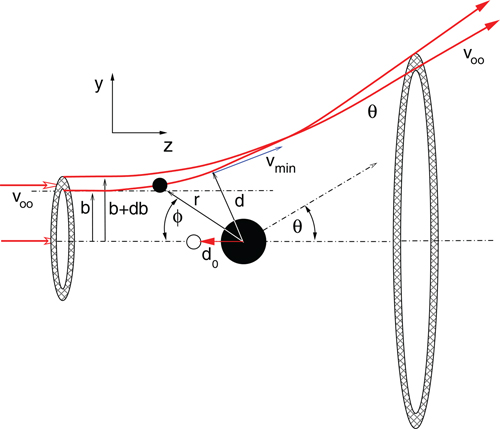
\includegraphics[width=0.6\linewidth, height = 6cm]{rutherford}
	\caption{Also know as rutherford scattering, a microscopic view of the scattering process (inside a foil for example).}
	\label{fig:rutherford}
\end{figure}
A term that may better fit than scattering cross-section, is \textit{angular differential scattering cross-section}.
We shall now try to define it.
Imagine we scattered ions through a thin foil and used at a distance $R$ away from the foil a detector with area $\Delta a$ at an angle $[\theta_c, \theta_c + \Delta \theta_c]$ where $\theta_c$ is the scattering angle of the ions that passed through the foil.
The thin foil will impact the ion with different impact parameter $b$ (this distance between the ion and the 'tangent atom', i.e., minimum interaction distance) and thus a different scattering angle.
The definition of this differential scattering cross section $dn_\theta$ is the number of ions scattered to the area $\Delta a$ (between  $[\theta_c, \theta_c + \Delta \theta_c]$) per unit time.
If $I_0$ is the flux of incident ions, the unit-less solid angle of the detector $\Delta \Omega$ is given by
$$\Delta \Omega = \frac{\Delta a}{R^2} = \frac{(R\Delta \theta_c) (R\sin\theta_c \Delta phi)}{R^2} = \Delta \theta \Delta \phi \sin\theta_c$$
The differential cross scattering would then be defined as $d\sigma (\theta_c)$ (normally in units of mm$^2$) and can be written with the help of the solid angle:
$$ \frac{d\sigma(\theta_c)}{d\Sigma} = \frac{1}{I_0} \frac{dn_\theta}{d\Omega} $$
The term on the LHS is the differential scattering cross section per unit solid angle, while on the RHS we have the inverse incident ion flux multiplied by the number of scattered ions into $[\theta_c, \theta_c + \Delta \theta_c]$ per unit solid angle and per unit time.
From Figure \ref{fig:rutherford} we see that the differential cross section can be written as $d\sigma = 2\pi b db$, thus the differential scattering cross section can be written
$$\frac{d\sigma (\theta_c)}{d\Omega} = \frac{b}{\sin\theta_c}\left|\frac{db}{d\theta_c}\right| $$
By measuring the scattering angle, we can get information of the impact parameter $b$.
So we can get really microscopic information just by measuring the scattering angle!
An important thing that happens during scattering is the transfer of energy, thus we must describe the \textit{energy transfer cross section}.
Image an ion beam with certain ion flux directed at a thin foil with target molecules.
The thickness of the foil is $\Delta x$ (extremely thin), where the area can be defined as a unit area.
Within the area you have scattering centers, the target atoms.
They can be defined as cross section areas $\sigma$.
We need a probability function to describe these scattering events dependent on the energy of the ions $E$.
We could then assume for $N$ scattering atoms per unit volume, we can calculate the number of target nuclei in our thin foil: $N \Delta x$ target nuclei (per unit area).
The total fraction of target nuclei in the surface area that act as scattering atoms is then $\sigma N \Delta x$.
All of this leads us to the probability $P$ that an ion with energy $E$ will undergo a scattering event:
$$P(E) = N\sigma(E) \Delta x$$
which can then be folowed up with the probability for transfer of energy $[T, T + dT]$ is
$$P(E, T)dT = \frac{dP(E)}{dT}dT = N \Delta x \frac{d\sigma (e)}{dT} = \frac{1}{\sigma (E)}\frac{d\sigma (E)}{dT}dT$$
The term $\frac{1}{\sigma (E)}$ is the total energy transfer cross section, and $\frac{d\sigma (E)}{dT}$ the differential energy transfer cross section.
This can be further calcualted in terms of impact parameter
$$\frac{d\sigma (E)}{dT} = \frac{4 \pi}{T_m} \frac{d\sigma (\theta_c)}{d\Omega} = \frac{4\pi}{T_m} \frac{b}{\sin\theta_c} \left| \frac{db}{d\theta_c} \right| $$
where $T_m = \frac{4m_1 m_2}{m_1 + m_2} E_u$ is the maximum transfer of energy during a scattering process.
The total cross section if the probability of impact is 1 can be calculated in terms of energy
$$\sigma (E) = \int_{T_{min}}^{T_{max}} \frac{d\sigma (E)}{dT}dT $$
or scattering angle
$$ \sigma (\theta_c) = \int_{b_{max}}^0 \frac{d\sigma (\theta_c)}{db}db =  \int_{b_{max}}^0  2\pi b db $$
but both are equivalent.
So that was a lot of basics for the understanding of ions in solids, and now we will actually apply this knowledge to calculate what will be the energy transfer during a whole path, what will be the damage, and ion energy range.

\section{Summary}\label{sec:summary3}

\begin{myitemize}
	\item samples have difficult potentials, so we can approximate using the leonard jones potential
	\item Depending on the energy of an ion, the interaction distance $r$ will change.
	For high $E$, we have low $r$, and vice versa for low $E$.
	\item Screening potential comes from the combination of Coulomb force with the Pauli exclusion principle at short distances, and the universal screening potential was discovered by Ziegler
	\item  Scattering is complicated but draw a picture and it should be fine.
    By measuring the scattering angle, we can determine microscopic properties of the interaction ($b$)
\end{myitemize}

%! Author = adam
%! Date = 28.02.21


\chapter{More Ion-Matter Interactions}\label{ch:more-ion-matter-interactions}
In the previous chapter, we covered the basics of ion-matter interactions.
This included the short- and long-range interaction of atoms and what forces govern in the various regimes, followed by the screening potential due to electrons.
Then we covered collisions of atoms and the scattering that occurs therewith.
Now we turn our attention to the following subjects:
\begin{myitemize}
	\item Ion stopping
	\item Energy loss processes
	\item Nuclear Stopping
	\item Electronic Stopping
\end{myitemize}

We want to now understand what it takes to stop an ion as it travels through a medium, as well as how to measure this quantity and receive valuable information therewith.
The application of ion stopping is important in areas such as radiation protection, ion implantation and nuclear medicine.

\section{Ion Stopping}\label{sec:ion-stopping}
The stopping power is a retarding force acting on charged particles due to the interaction with matter resulting in a loss of particle energy.
The stopping power $S$ can be written as the energy loss per unit length:
\begin{equation}
S(E) = -\frac{dE}{dx}\label{eq:stopping}
\end{equation}
and takes on a value of $\approx 100$ eV/mm (in SI units it is Newtons).
The penetration depth $R$ can be then calculated using $E_0$ the initial kinetic energy of the particle:
\begin{equation}
R = \int_0^{E_0} \frac{1}{S(E)}dE
\end{equation}
A way to visualize this is to imagine an ion scattering within a sample, and each time it collides randomly, it is deflected and travels a distance $r_i$ before randomly colliding again, traveling a new distance $r_i$. $R$ is then $R = \sum_i r_i$.
There are two main different energy loss processes that can stop an ion that we will consider.
In nuclear stopping, we have large discrete energy losses for each collision that result in significant angular deflection.
For electronic, there is much smaller energy loss per collision, and negligible deflection.
Together we get the following inelastic collision formula:
This can be seen in Figure~\ref{fig:ionstop}
$$ \frac{dE}{dx} = \frac{dE}{dx} |_n + \frac{dE}{dx}|_e $$
We can further define the \textit{stopping cross section} as $$S_n = \frac{dE}{dx} / N$$ where $N$ is the atomic density and $S_n$ has units of [eVcm$^2$/atom].
This quantity can be understood as the energy loss rate per scattering center.
At low ion energies (low frequency of ion), nuclear stopping dominates, but as we reach higher impact particle energies, we electric stopping dominates.

\begin{figure}
	\centering
	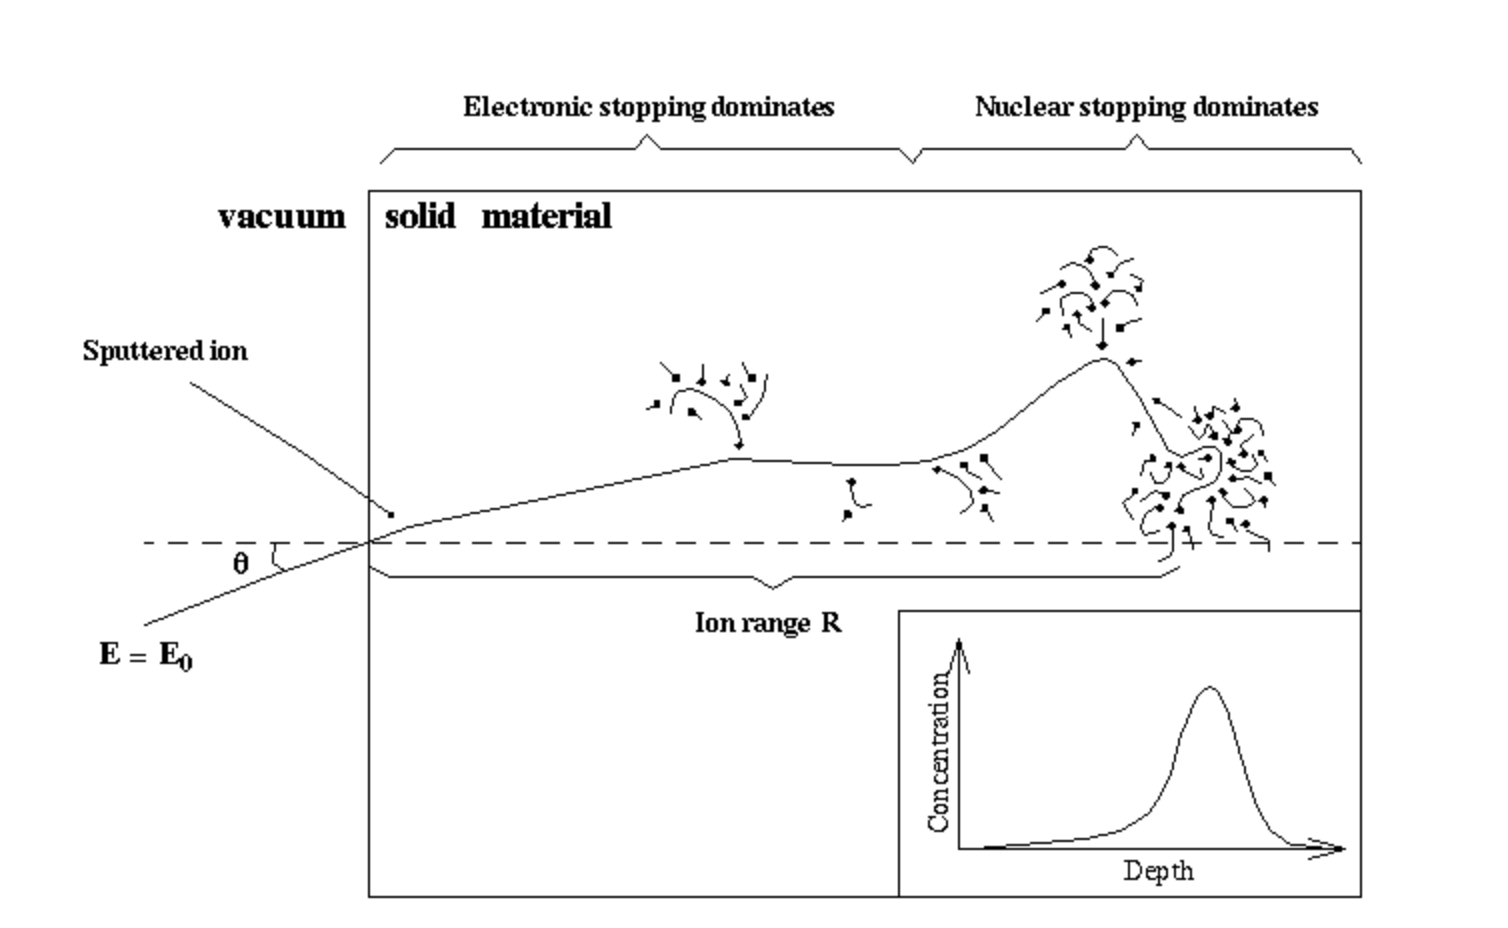
\includegraphics[width=0.6\linewidth, height=6cm]{ionstopping}
	\caption{General picture of ion stopping. Sputtering will be covered in the future.  In the beginning of the slowing down process at high energies, the ion slows down mainly by electronic stopping, and moves almost in a straight path. When the ion has slowed down sufficiently, the collisions with nuclei become more and more probable, finally dominating the slowing down. \cite{4}}
	\label{fig:ionstop}
\end{figure}

\section{Nuclear Stopping}\label{sec:nuclear-stopping}
Nuclear stopping power or the nuclear energy loss rate is the energy loss by a moving ion due to elastic collisions per unit length traveled within the target.
The word nuclear may cause confusion because nuclear stopping is not in fact due to the nuclear forces, but rather is meant to note that this stopping involves the interaction of the ion with the nuclei in the target.
We can then calculated the average energy loss using the probability of a collision for a given energy range: $$ \langle dE \rangle = \int T \frac{dP(E)}{dT}dT = N \int_{T_{min}}^{T_{max}} T \frac{d\sigma (E)}{dT}dTdx$$
For infinitesimal $dx$ we receive the nuclear stopping power $$ \frac{dE}{dx} |_n = N \int_{T_{min}}^{T_{max}} T\frac{d\sigma(E)}{dT}dT$$ where $T_m$ is defined in previous chapters and is the maximum energy transfer.
Using the nuclear stopping power defined above, we can easily calculate the nuclear stopping cross section $S_{nn}$ is defined similarly as before.

\begin{equation}
	S_{nn} = \frac{1}{N} \frac{dE}{dx}|_n = \int_{T_{min}}^{T_{M}} T \underbrace{\frac{d\sigma (E)}{dT}}_\textrm{ETDCS} dT
\end{equation}

The term ETDCS stands for energy transfer differential cross section.
\subsection{ZBL Model}\label{subsec:zbl-model}
To model the nuclear stopping cross section $S_{nn}$, we can use the previous screening potential from Ziegler, Biersack and Littmark, to get something like $S_{nn}^{ZBL}$
A lot of the time this ZBL model is used in computer simulations for binary collision approximations, one being \href{http://www.helsinki.fi/~knordlun/TRIM-answer}{TRIM}.
The ZBL approximation for the nuclear stopping cross section fits experimental results for low and high energies, and although it is a quite complicated function we will not write here, it is general knowledge in approximating ion nuclear stopping.
\section{Electronic Stopping}\label{sec:electronic-stopping}
At low energies (low velocities), the electronic stopping power $S_{ne}$ has a low impact, but as velocities increase, it will also increase.
We can see in Figure~\ref{fig:ionstop2}, the electronic stopping power starts to decrease again.
This decrease can be characterized with $v > v_0 Z_1^{2/3}$, as the ion becomes fully stripped of all of its electrons.
The ion can be then considered in a charge state $Z_1$ (the atomic number of the ion) since it fully looses its electrons.
A collision causes a sudden transfers energy from the ion to the target electron, as the velocity of the ion is much higher than the orbital electron.
The orbital electron (in the sample) can be regarded as a quasi-stationary particle (in comparison to the ion).
Therefore we can calculate the energy loss from scattering in a central force field!
In very high energy regimes, $S_{ne} \propto \left( \frac{Z_1}{v}\right)^2$
\begin{figure}
	\centering
	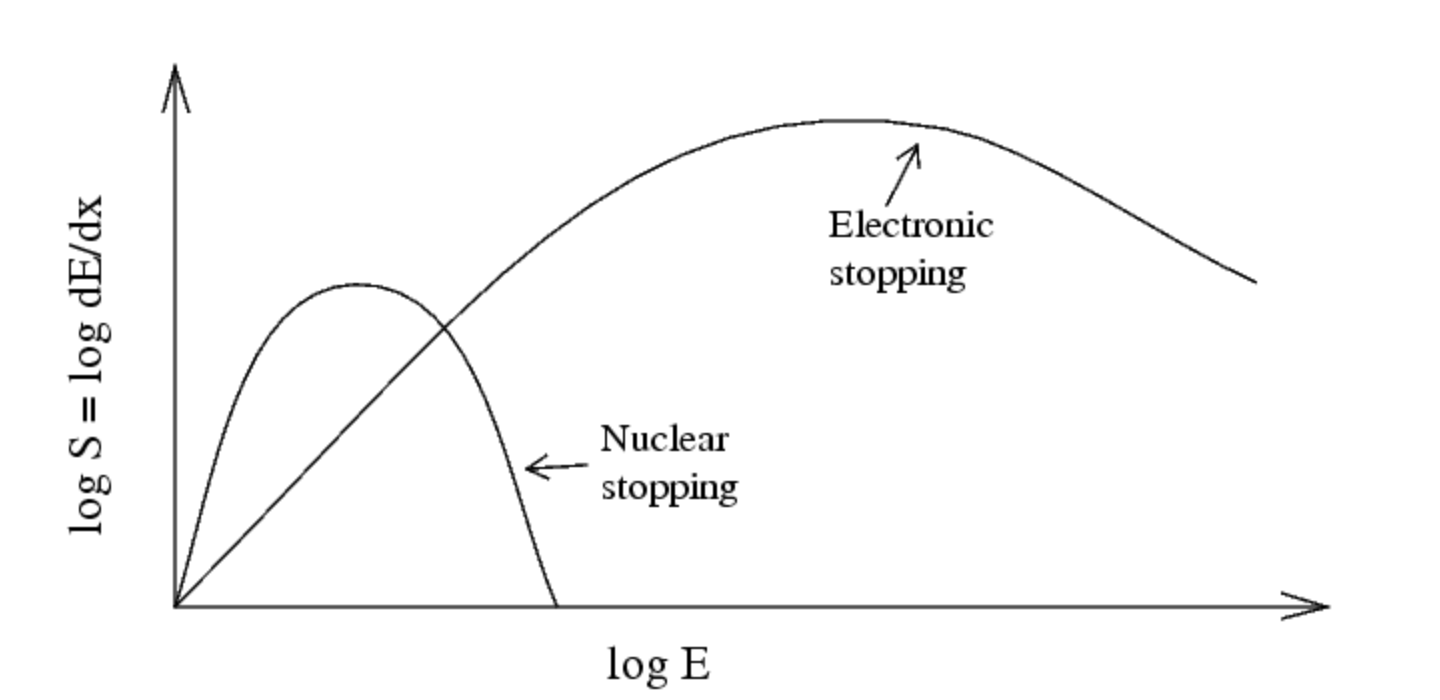
\includegraphics[width=0.6\linewidth, height=5cm]{ionstop2}
	\caption{Ratio between nuclear and electronic stopping power. The maximum of the nuclear stopping curve typically occurs at energies between 10--100 keV, of the electronic stopping power at MeV energies. For very light ions slowing down in heavy materials, the nuclear stopping is weaker than the electronic at all energies. \cite{4}}
	\label{fig:ionstop2}
\end{figure}

\subsection{Low Energy Regime}\label{subsec:low-energy-regime}
For $v < v_e$ we have a linear expression for $S_{ne}$.
There are several models to get this result, but all models converge to $S_{ne} \propto v$.
Two examples of these models are Firsov, where the ion loses a small amount of momentum if it picks up an electron, and the Linard-Scharff formula, which is written as with some pre-factor $K$ such that: $$S_{ne} \propto K \sqrt{E}$$
\subsection{High Energy Regime}\label{subsec:high-energy-regime}
At high energy, the ion is a bare nuclei and loses all of its electrons, and therefore has the pure coulomb potential from the target atoms.
Bohr calculates this classically, as the electron is basically not moving in comparison to the ion that flies by.
However, at high energies we must take into account the relativity effects, as well as the shell structure of the atom's electrons, and the QM effects.
This is called the Bethe-Bloch Formula.
The end results I write below, where first we see the Bohr expression for the electronic stopping power (classical)
\begin{equation}
	\frac{dE}{dx} \propto \frac{1}{E} \ln \frac{E}{E_B}\label{eq:borh}
\end{equation}
This is derived using a combination of Gauss law for a moving ion and stationary electron with Coulomb interaction to determine the change in momentum of the ion, and thus the change in energy.
and then the Bethe-Bloch Formula (including relativistic effects) for the electronic stopping power
\begin{equation}
	\frac{dE}{dx} = -\frac{Z_1^2 e^4 n_e}{4\pi \epsilon_0^2 v^2 m_e}\left[ \frac{1}{2} \ln \left( \frac{2m_e v^2 \gamma \Delta E_{max}}{I^2}\right) - \beta^2 - \frac{\delta}{2} - \frac{C}{Z_2}\right]\label{eq:beathe}
\end{equation}

\section{Summary}\label{sec:summary4}
The impact of ions on samples is quantified using \textit{stopping power}, which has components nuclear and electronic.
The ions can remain stuck in the sample because of this, and this stopping regime explains sputtering.
\begin{myitemize}
	\item As an ion penetrates a sample, there are different mechanisms that make the ion 'lose' energy as it collides with other atoms within the sample
	\item Nuclear stopping involves elastic collisions, and results in large discrete energy losses resulting in large angular deflection
	\item Electronic stopping involves inelastic collisions, and results in smaller energy loss per collision, thus negligible deflection.
	\item High energy electronic stopping is governed classically by coulomb potential, $S_{ne} \propto \left( \frac{Z_1}{v}\right)^2$, but exact solutions need to consider relativistic effects (Beathe-Bloch Formula)
	\item Low energy electronic stopping we have linear proportionality to velocity (thus $\propto \sqrt{E}$)
\end{myitemize}

%! Author = adam
%! Date = 28.02.21


\chapter{Ion Range and Impact on Solid State Computer Design}\label{ch:ion-range-and-impact-on-solid-state-computer-design}
In this chapter we will examine the following topics:
\begin{myitemize}
	\item Ion Range
	\item Displacements/Damage
	\item SRIM Simulation
	\item Channeling
\end{myitemize}

We want to build the connection of the previous chapter to the ion range, i.e., the range or depth in which the ion enters the sample.
The Figure~\ref{fig:ionstop} gives a visualization of the depth of which the ion goes in the solid.
For high energy particles or low mass ions, the electronic stopping dominates, and the low energy nuclear dominates.
For heavy ions (lead for example), there will always be a domination of the electronic stopping, i.e., the range depends heavily on the mass and energy of the ion.
Ion range has a great practical importance for radiation therapy, as we will see later when it comes to Bragg Peaks.

\section{Ion Range}\label{sec:ion-range}
We first have to define a bit of terminology in which we can discuss the depth of the ion entering into the sample.
Imagine a surface plane of a material in a coordinate system of your choosing.
An ion then impacts the beam with a certain angle $\alpha$ relative to the normal of the surface of the plane.
Due to elastic collision, we will not have a straight path through the sample of the ion, but rather a jagged path.
There are different definitions of the ion range, one most discussed is called the \textit{projected range} $R_p$.
This is the projected distance in which the ion would go if it was not deflected.
The \textit{transversal projected range}, $R_p^t$, is the length between the real end point of the ion normal to the projected range.
The direct distance between the point of rest and the point of incident is the \textit{radial range}, $R_r$.
Imagine now we take the point of rest, and we take a projection of this point to the surface plane.
The distance from this point on the plane to the incident point is called the spread, $R_s$.
Since we have a certain angle of incident, the radial range is not the same as the penetration depth of the ion, therefore the depth $x_s$ is normal to the surface plane.
Definitions of the various terms are given below, where the point $(x_s, y_s, z_s)$ is the point in which the ion stops (in cartesian coordinates) beneath the sample surface plane.

\begin{gather*}
    R_s = \left( y_s^2 + z_s^2 \right)^{1/2}\\
    R_r = \left( x_s^2 + y_s^2 + z_s^2 \right)^{1/2}\\
    R_p^t = \left[ \left( x_s \sin(\alpha) - y_s\cos(\alpha) \right)^2 + z_s^2 \right] ^{1/2}\\
    R_p = \left[ R_r^2 + R_p^{t2}\right] ^{1/2}\\
\end{gather*}
If $\alpha = 0$, $R_p = x_s$, and $R_s = R_p^t$.
\subsection{Distribution}\label{subsec:distribution}
Discussed above is the case for a single ion, but since we use ion beams normally, this will result in some sort of distribution since stopping is a random and thus stochastic process for each individual ion.
The total ion path length will then be different for each ion, i.e., statistically broad distributions of ion penetration depth.
This range distribution, also called the \textit{straggling}, can be quantified using the density of particles $N$ given the depth within the sample $x$, $\rightarrow N(X)$:
\begin{equation}
	N(x) = \frac{\Phi_i}{\Delta R_p \sqrt{2\pi}} exp \left[ -\frac{1}{2} \left( \frac{x - R_p^2}{\Delta R_p}\right) ^2\right]
	\label{eq:struggle}
\end{equation}
where $\Delta R_p$ is the projected range straggling, and $R_p$ is the projected range (mean depth). $\Phi_i$ is called the fluency, and is defined,  $\Phi_i =  \int_{-\infty}^\infty N(x)dx$.
From~\ref{eq:struggle}, we can see that $N(R_p) = N_p = \frac{\Phi_i}{\Delta R_p 2\phi}$
One would end up with a gaussian distribution for $N(x)$, with maximum at $x = R_p$, with the FWHM being equal to $2 \Delta R_p$
Normally, for 100 kV Boron implanted into Silicon, the mean penetration depth will be about 380 nm, but with straggling of mostly 90 nm.
Usually, one would use $1/$cm$^2$ for a unit of fluency, therefore straggling will also have units of cm.
$N_p$, the number of ions at mean penetration depth will be in units of atoms per cm$^3$.
For all other quantities related to the range, i.e., depth or longitudinal range, can also be distributed using this method.

\subsection{Bragg Peak}\label{subsec:bragg-peak}
We see that the energy loss per unit distance increases as the particle slows down.
The curve describing this fact is the Bragg curve.
Shortly before the end, the energy los passes through a maximum, the \textbf{Bragg Peak}, then drops to zero.
More is discussed in~\ref{fig:bragg}.
This is used in cancer treatment.
This is fantastic, since we know that for high energy, there will be low energy deposition at the beginning of the depth, followed by an extremely high increase in interaction and nuclear stopping at the end.
\begin{figure}
	\centering
	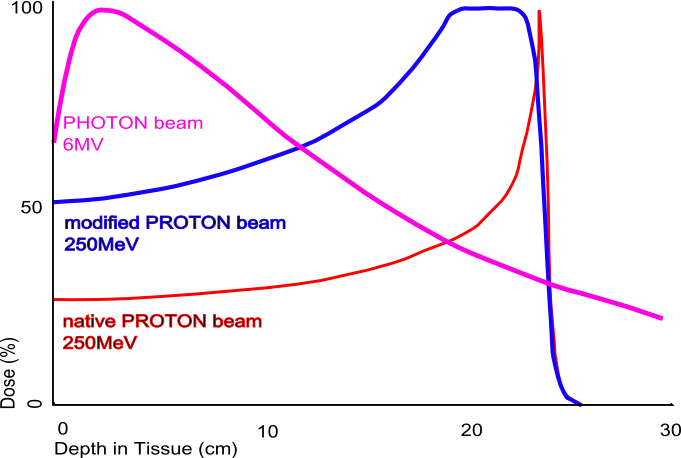
\includegraphics[scale=0.4]{BraggPeak}
	\caption{Here we have various proton beams, with increasing energy, as a function of depth within the tissue. For a native Proton beam, we have a low loss of energy due to the electronic stopping, and therefore an increase in interactions, and finally a peak in the energy interactions at a certain position, called the Bragg peak.}
	\label{fig:bragg}
\end{figure}


\section{Displacement and Damage}\label{sec:displacement-and-damage}
Not only is the path of the ion important, but also the displacement of atoms within the sample due to the ion important.
The type of motion exhibited by the atoms is modeled by a phenomena called cascade.
There are some nice videos on youtube (\href{https://www.youtube.com/watch?v=HNFwXnGmie4}{example}), where we see that the ion collides with an atom, called the \textit{primary knock on atom}, which then goes on to cause a cascade of other collisions with other atoms within the sample.
The displacement threshold, or energy, in which a collision would occur is denoted by $E_d$, this is the minimum energy that an ion (or atom in the case of it being already displaced and is moving to displace other atoms) must have in order to displace an atom from its lattice site.
We consider two temperature ranges, one below the threshold and one above.
For $T < E_d$, there is a vibration as the atom that was struck by the ion quickly shares its energy with the nearest neighbor atoms, i.e., a local heat source.
For $T > E_d$, it is a displaced atom, i.e., the simplest case, and the atom is deflected just like how an ion would be deflected, leading to vacancy-interstitial pairs (Frenkel pair) in the atomic structure due to the displaced atom.
But, we can only really define an average $ \langle E_d \rangle $, since $E_d$ depends on direction.
For example, the $ \langle E_d \rangle $ for Silicon is around 16eV, and for Aluminum 43 eV.

\subsection{Kinchin-Pease Model}\label{subsec:kinchin-pease-model}
Let's assume we have the energy of the primary knock on (PKA) atom, which has energy $E_\nu >> E_d$, so the PKA will have many more recoil atoms and displacements following from it.
This displaced atoms can in turn displace additional atoms.
At the end we will end up with many collisions and displacement events which occur in proximity with each other.
Therefore we can introduce the \textit{displacement damage function}, $\langle N_d (E) \rangle $, which of course depends on the energy of the PKA.
This is just the average number of displaced atoms in a cascade produced by a PKA.
The simplest model for this is the Kinchin-Pease model, based on a hard sphere model, where the nuclei of the atoms are assumed to be hard spheres.
The KP model has the following assumptions, which turn out to be good enough for approximations.

\begin{myitemize}
	\item Collision between like atoms,  i.e., $M_1 = M_2$
	\item Hard-sphere cross section, i.e., $P(E,T)dT \approx \frac{dT}{E}$
	\item Cascade of two body collisions, (binary collision approximation)
	\item Elastic nuclear collisions
	\item $E_d$ neglected in energy balance of elastic collision
	\item No crystal structure
	\item $T < E_d \rightarrow $ no displacement
	\item $E < E_d$ for a knock-on atom $\rightarrow $ no further contribution to cascade
	\item atoms receiving $E_d< E < 2E_d$ are displaced but can not themselves further increase the total number of displacements
\end{myitemize}
In the Kinchin-Pease model the number of point defects generated by an implanted ion is derived analytically from the energy that is transferred from an ion to an atom of the target material.
It is assumed that the number of point defects generated by a primary recoil is proportional to the energy transfered from the ion to the primary recoil.
A primary recoil is a recoil generated by the collision of an implanted ion with a target atom, while secondary recoils are generated by recoils.
Using this we can approximate the number of Frenkel pairs $N_d$ generated by a PKA atom.
$$ \langle N_d (E_\nu) \rangle = \begin{cases}
			 0 & E_\nu < E_d \\
			 1 &  E_d < E_\nu < 2E_d \\
			 \frac{E_\nu}{2E_d} & 2E_d < E_{\nu} < E_c \\
			 \frac{E_c}{2E_d} & E_{\nu} > E_c
\end{cases} $$

Here, we detail the above relations.
For the first case, it is obvious that there will be 0 point defects for an energy less than the displacement energy.
For the second relation, we will have a total of 1 displacement for energies between $E_d $ and $2 E_d$, from which there are two possibilities.
The PKA can cause a collision with another atom, which the transmitted energy could be $E_d < T < 2E_d$, and the lattice atom will be displaced.
The initial PKA is then left with an energy less than the displacement energy, therefore the initial PKA is left with $E_\nu < E_d$, so no stable Frenkel pair, and the PKA falls into the vacant site left by the displaced atom.
This is called a \textit{replacement collision}, and is more probable than a permanent replacement.
For a transmitted energy $T \rightarrow T < E_d \Rightarrow$ lattice atom will \textunderscore{not} be replaced.
The primary PKA atom is left with insufficient  $E_\nu$ for other displacement.
In both cases we are moving one atom which has less energy than the initial PKA.
Therefore with PKA with energy between $E_d$ and $2E_d$ we will leave with only one displaced atom.
For mono-atomic samples, these two cases make really no difference, but with multi-atomic samples we can change which atom is at which lattice site.

Now we can ask what happens for $E_\nu > 2E_d$.
We have to calculate the average recoil energy $\langle T \rangle $ produced by a PKA with energy $E_\nu$.
$$ \langle T =  \rangle \int_0^{T_M} T P(E,T) dT = \frac{1}{T_M} \int_0^{T_M} TdT = \frac{E_\nu}{2} $$
The $P(E,T)$ term comes from the hard sphere cross section assumption, and is the probability of a certain transfer energy to occur, and $PdT = dT / E$.
The maximum transfered energy possible $T_M$ is really just the energy of the atom $E_\nu$.
Finally, this leads us to be able to calculate the average number of displacements produced by a mean recoil energy, $\frac{\langle T \rangle}{E_d} = \frac{E_\nu}{2E_d}$

But for high energies $T$, we will have some diversion, so we define the critical energy $E_c$ to take into account the electronic losses of PKA.
It is just the mass number of the element times 1 keV, i.e., $E_c = M_2$keV. The typical value of $E_c $ for copper is $62$ keV.
For PKA's with $E > E_c$, the distribution can be written as a constant value:
$$\langle N_d (E_\nu) \rangle  = \frac{E_c}{2E_d}$$


\section{Let's Build a Solid State Quantum Computer}\label{sec:let's-build-a-solid-state-quantum-computer}
A very short introduction to the criteria for a SSQC. We need to fulfill these criteria in order to build one, and were defined by Divencenzo.
Initially there were just five conditions, but if we want to do quantum communications we need the last two.
\begin{enumerate}
	\item A \textbf{scalable} physical system with well characterized qubit
	\item The ability to \textbf{initialize} the state of the qubits to a simple fiducial state
	\item Long relevant \textbf{decoherence} times
	\item A "universal" set of quantum \textbf{gates}
	\item A qubit-specific \textbf{measurement} capability
	\item The ability to \textbf{interconvert} stationary and flying qubits
	\item The ability to faithfully \textbf{transmit} flying qubits between specified locations
\end{enumerate}
In the context of ion implantation, there are two things that are important, as the technique of implantation will directly correlated scalability and decoherence.
Scalability means that we will not only have to be able to produce one qubit, but rather multiple qubits.
Decoherence time should be very long so that we can actually use these qubits.
The implantation needs to be deterministic, i.e., if we want to implant an ion in a sample, we need to be sure that we can do this with however many ions we want to put there.
Some questions to consider before reading on:
\begin{myitemize}
	\item What could be the bottleneck of ion beam techniques and what are the advantages for building a solid-state quantum computer?
	\item What are the challenges?
\end{myitemize}


\section{Summary}\label{sec:summary5}

\begin{myitemize}
	\item With ion beams, the scattering of the ions within the sample is a stochastic process, and can be modeled using distribution functions
	\item Straggling is the distribution of these ions due to the stochastic processes, and has a major impact in the building of a quantum computer in the solid state.
	\item Bragg peaks define where in the penetration depth a high increase in transmitted energy will occur
	\item KP model is a simple set of assumptions to help describe how atoms will interact with each other depending on their energies after being struck by a penetrating ion or atoms that were first struck by the ion (PKA's)
	\item Ion implantation physics like straggling have a great influence on theoretical quantum computers, as if we wanted to create qubits we would find restrictions like $E \leq 10 keV$ to not allow for straggling to take over spatial resolution.
\end{myitemize}


%! Author = adam
%! Date = 28.02.21

\chapter{Channeling}\label{ch:channeling}

Last chapter we discussed the stochastic process of a ion beam as it collides with atoms within a crystal/sample.
But what happens if the incident beam of ions is perfectly aligned in the 'gaps' of a crystalline lattice?
The german word for this phenomena I think fits quite well: Gitterfuehrungseffekt, i.e., to pass through the lattice.
A diagram of when this is to happen is found in Figure~\ref{fig:channel1}.
Basically, the ion is constrained on its path through a crystalline solid.
This is not the case for amorphous solids (non crystalline) as there we would have the effects described in the previous chapter.
\begin{figure}
	\begin{subfigure}{0.5\textwidth}
		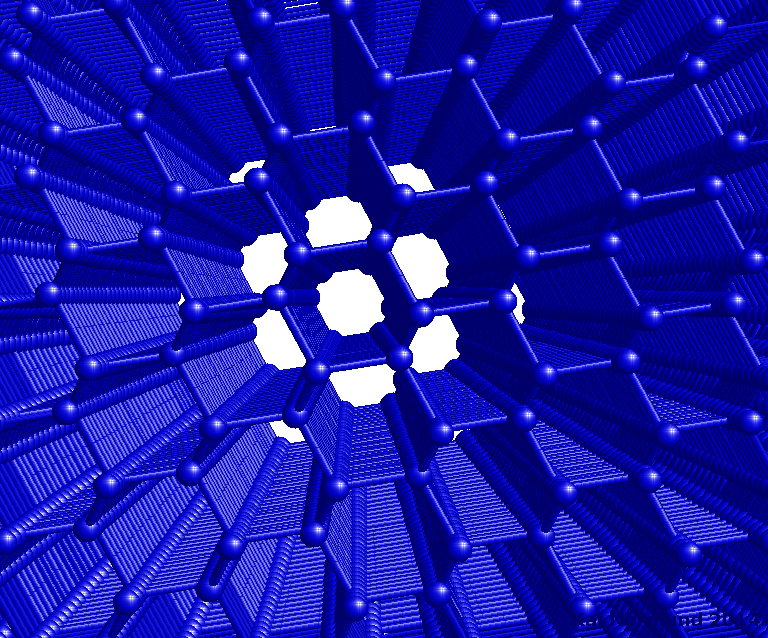
\includegraphics[width=0.9\linewidth, height=5cm]{SC1}
		\caption{An about 12 nm thick silicon crystal viewed down the 110 crystal direction.}
		\label{fig:SC1}
	\end{subfigure}
	\begin{subfigure}{0.5\textwidth}
		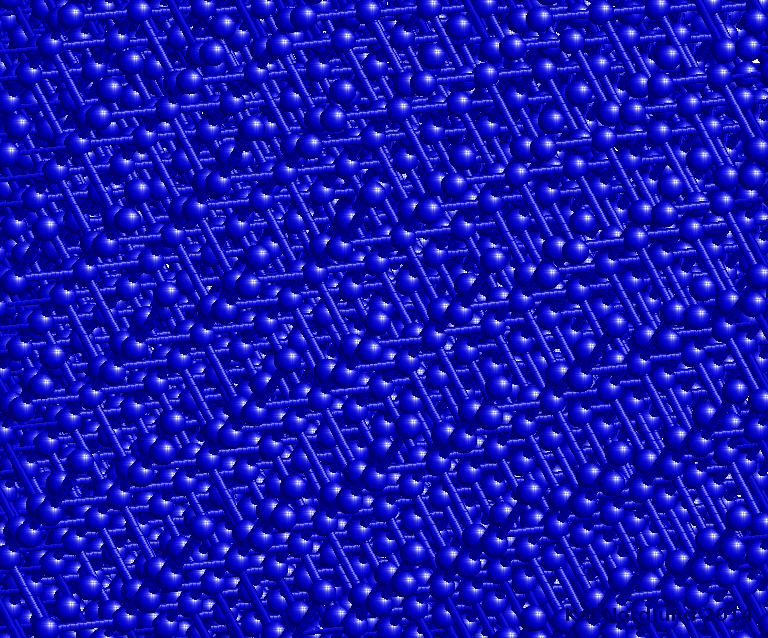
\includegraphics[width=0.9\linewidth, height=5cm]{SC2}
		\caption{The same Si crystal, but viewed from a randomly rotated direction}
		\label{fig:SC2}
	\end{subfigure}
	\caption{POV of an ion coming to hit a crystal from two different angles. Taken from wikipedia}
	\label{fig:channel1}
\end{figure}
 The influence of the crystal lattice not only appears in the orientation of the lattice, but also in the vibrational amplitude of the lattice atoms (T).
Additionally, properties like surface preparation, beam divergence, and disorder introduced by the implantation itself can lead to changes in the channeling effect.

In channeling, we have a much lower energy loss, i.e, stopping power.
This leads to a greater range in which the particle can travel through the sample.
Due to this, we have less resulting nuclear stopping, and thus less damage to the sample.
\section{Continuum Model}\label{sec:continuum-model}
Also called axial channeling, the continuum model
The trajectory of a channeled particle is described mathematically below but schematically in Figure~\ref{fig:trajec}

\begin{figure}
	\centering
	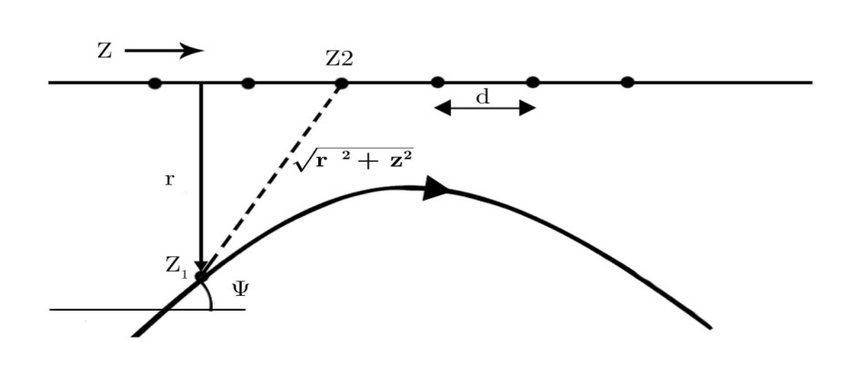
\includegraphics{trajectory}
	\caption{Trajectory of a channeled particle}
	\label{fig:trajec}
\end{figure}
As they travel through the 'channel', ions feel a screened potential, $U$,  given by:
$$U(r) = \frac{Z_1 Z_2 e^2}{4\pi\epsilon_0 d} \ln \left[ \left( \frac{\sqrt{3}a}{r}\right)^2 + 1\right]$$
where $d$ is the spacing between atoms within their planes, $a$ is the Thomas-Fermi radius.
We can use conservation of energy to determine the critical angle $\Psi_c$ between the plane between two planes in which the ion will oscillate around.
$$ E = \frac{p_{\parallel} ^2}{2m} + \frac{p_{\perp} ^2}{2m}  + U(r)$$
where $p_\parallel = p\cos\Psi$, $p_\perp = p\sin\Psi$.
This yields us:
$$ E = \frac{p^2 \cos^2 \Psi}{2m} + \frac{p^2 \sin^2 \Psi}{2m} + U(r)  \underbrace{\rightarrow}_{\Psi << 1} \frac{p^2 \Psi^2}{2m} +  \frac{p^2 \Psi^2}{2m} + U(r) \underbrace{\rightarrow}_{\textrm{perp. part}}  E_\perp \approx \frac{p^2\Psi^2}{2m} + U(r) $$
Th minimum distance $r_m$ where the channeling breaks down (i.e., where $\Psi_c$ is), is then:
$$ \frac{p^2\Psi_c^2}{2m} = E\Psi_c^2  \overset{!}{=} U(r_m) \Rightarrow \Psi_c = \sqrt{\frac{U(R_m)}{E}}$$
How do we find $r_m$? If $r_m$ is approximately in the range of the thermal vibrational amplitudes of lattice atoms then the channeling breaks down.
Therefore if we assume \textunderscore{isotropic} thermal amplitudes, then the mean square vibrational amplitude $\langle u^2 \rangle$ will yield us:
$$r_m \approx \rho = \sqrt{\langle x^2 \rangle + \langle y^2 \rangle} - \sqrt{ \frac{2}{3} \langle u^2 \rangle} $$
and finally:
$$\Psi_c = \sqrt{\frac{2Z_1 Z_2 e^2}{4\pi \epsilon_0 d E}} \sqrt{\frac{1}{2} \ln \left( \frac{\sqrt{3} a}{\rho}\right) + 1}$$
Since $a$ is normally on the order of 0.01 mm, and $\rho$ on the order 0.005 mm, then the right square root is approximately 1.

The continuum model can be broken down into three broad categories.
Group \textbf{A}: There is strong interaction with the lattice, and the range distribution is similar to that of an amorphous material.
Group \textbf{B}: the ion starts with large oscillations in the channel, followed by a high probability to be de-channeled at some point.
Group \textbf{C}: these ions are 'well' channeled, i.e., there is a good chance to remain channeled during the whole slowdown process.
How does an ion beam join one of these three groups?
Well for that we have a little table:

\begin{table}[h]
	\centering
	\begin{tabular}{c | c | c }
		\hline
		Group & Angle & Position \\
		\hline
		A & $\Phi_A > \Phi_C$ & close to atomic rows \\
		B & $\Phi_B < \Phi_{cr}$ & slightly further away to atomic rows \\
		C & $\Phi_C < \Phi_B < \Phi_{cr}$ & near the channel center
	\end{tabular}
	\caption{The angle is that relative to the midline between the two crystal lattice planes.  }
    \label{tab:Continuum}
\end{table}
Dechanneled, which just means that the ion, either abruptly or at the end of its range, leaves its channeled path.
This can occur at any point during the channeled ions' life, i.e., there is a probability for it to just de-channel, and in some cases it is more likely to do so than other (see group B of continuum model).
There are some maximum ranges that come with channeling, if we have a 50--150 keV ion beam and good alignment to the main crystal axis, then the range of the ion depth is 2--50 times greater than that of an amorphous solid!
Also, the stopping of channeled ions (de-channeling) is determined by electronic stopping.
If we recall from previous chapters, near the end of the ions' life in the sample, this is where electronic stopping occurs.
This leads us to the stopping power relations of:
$$\underbrace{S_e}_\textrm{channeled} << \underbrace{S_e + S_n}_\textrm{amorphous} $$
where $S_e$ and $S_n$ are the electronic and nuclear stopping powers respectively.

One can also use de-channeling to investigate defects of samples.
Imagine the rows of atoms are not so neat, and we were to have some defects, i.e., atoms are not aligned on the plane.
If we were to have one of these defects, then the channeling that was to be assumed to be fine, there would in fact be maybe a backscattering event, or the ion becomes de-channeled and is no longer in the crystal channel.
One can measure the proportion of the beam that is channeled vs not channeled (scattered for example), we can learn something about the crystal quality, and the defects relative to the crystal.
This can be seen in Figure~\ref{fig:dech}

\begin{figure}
	\centering
	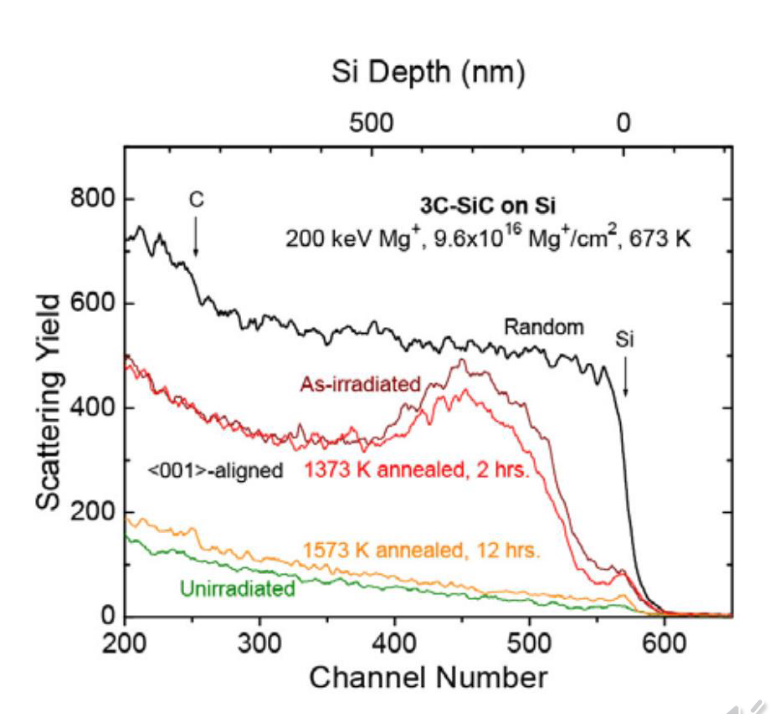
\includegraphics[scale=0.35]{dechannel}
	\caption{Here we have a silicon sample with various types of defects implemented in the sample that is being fired upon with a 200 keV helium beam ion. On the y-axis we have the backscattered ions, and the x-axis the number of channeled ions. The black line (random) is with random orientation of the ion beam so we have high number of back scattered atoms. For an non irradiated sample without any disorder, we have a low number of backscattered ions. Annealing is discussed later chapters but we note here that over a time, the annealing repairs the damage from the implantation (red lines) such that we are back to having a high amount of channeled atoms compared to those backscattered.}
	\label{fig:dech}
\end{figure}

\section{Example: Diamond}\label{sec:example:-diamond}
In Leipzig there is a lot of work done using diamond, which has two crystal planes that work well for channeling: $\langle 100 \rangle$ and $\langle 111 \rangle $.
After plugging in numbers from literature, we can find our $\Psi_c \approx 6^{\deg} $ for E$\approx 200$keV of an Argon ion beam in Diamond.
\section{Summary}\label{sec:summary6}
\begin{wrapfigure}{r}{0.5\textwidth}
	\centering
	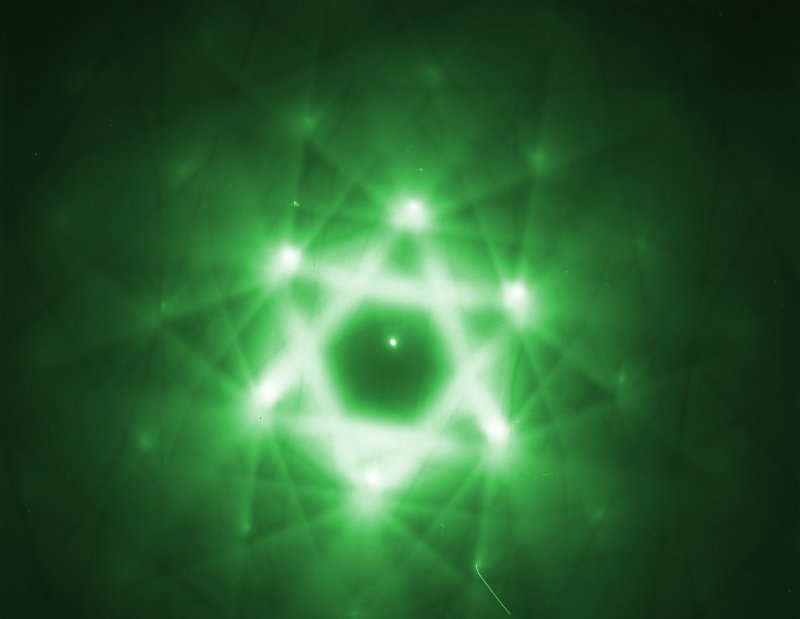
\includegraphics[scale=1.3]{BZ_ion}
	\caption{The brillouin zone construction by 300keV electrons. }
\end{wrapfigure}
Fun fact this was discovered initially through computer simulations.
There are several interesting application of channeling.
Channeling effects can be used as tools to investigate porerties of the crystal lattice and of its perturbations (like doping) not accessible to X-rays.
It may also be utilized to detect geometrical abnormalities in crystals, and is a variation of Rutherford Backscattering.
Channeling can even super-focus ion beams for sub-atomic microscopy.
At higher energies (tens of GeV), the applications include channeling radiation for enhanced production of high energy gamma rays, and the use of bent crystals for extraction of particles from particle accelerators.

\begin{myitemize}
	\item If ions hit at just the right angle to a crystal lattice, then they will be channeled, i.e., will follow a relatively linear path without being scattered and displacing other atoms
	\item There are three main groups of ions impact that result in scattering, based off of angle and the position relative to crystal plane
	\item Channeling is due to the Coulomb potential felt by the ion as it travels between the plane, leading it to an oscillatory motion.
\end{myitemize}

%! Author = adam
%! Date = 28.02.21

\chapter{Ion Beam Methods}\label{ch:ion-beam-methods}
\epigraphfontsize{\small\itshape}
\epigraph{ ``It was quite the most incredible event that has ever happened to me in my life. It was almost as incredible as if you fired a 15-inch shell at a piece of tissue paper and it came back to hit you''}{--- \textup{Ernest Rutherford}, \cite{2}}
Now lets see if instead of penetrating a sample, we scatter away from it.
An important term here is the \textit{scattering cross-section}, which is the probability of an ion-solid interaction.
\textit{The differential cross-section}  gives us a measure of either the probability of transferring energy $E$ in range $[E, E + dE]$ or the probability of scattering into angle $[\theta, \theta + d\theta]$. If we integrate the differential cross-section overl all $\theta$, we recieve a value called the \textit{total cross-section} Most of the time the scattering cross section is given in units of mm$^2$.
A diagram to better understand the microscopic scattering cross section is found in Figure~\ref{fig:rutherford}.

\begin{figure}
	\centering
	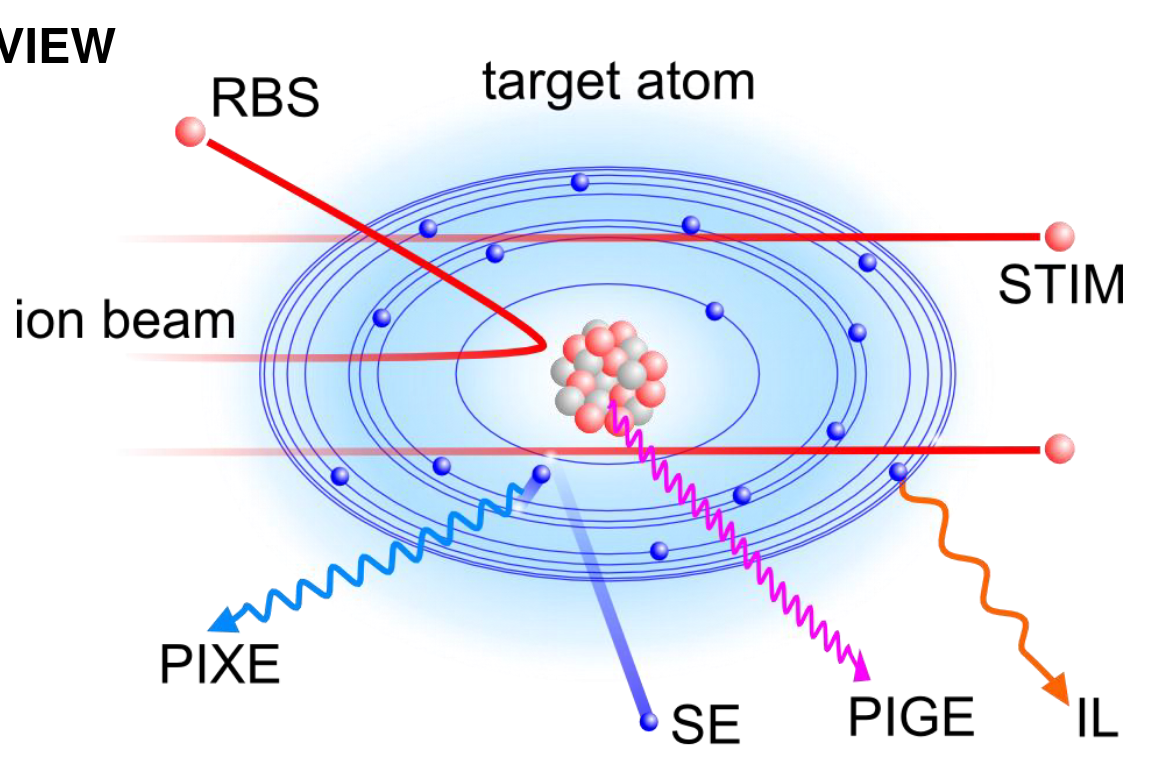
\includegraphics[width=0.7\linewidth, height=6.5cm]{overview}
	\caption{Various reactions of an ion beam hitting a target atom. The target atom has a nucleus and atomic shell, from which we can receive valuable information depending on how the beam interacts. STIM is the transmission of the ion through the sample, used in scanneing tunneling microscopy. }
	\label{fig:over}
\end{figure}
In this chapter we want to see how we can use ion beams to analyze samples.
These techniques are used in Leipzig, and we can see how some of these classical methods of ion beams can be used for quantum technologies.
First we need to see the difference between electron and proton radiation.
With electrons, we normally have large angle scattering, as well as not so deep range into the sample.
For protons, at the beginning of the trajectory there is not as much straggling as the electron, followed by a Bragg peak at the end.
Along the path there is very limited straggling, and the spatial resolution is high in comparison to the electron beams.
The penetration depth is also comparatively larger.
Now we want to see and discuss protons interacting with a solid in order to do analysis of the solid.
A general overview of the different ion beam methods is given in Figure \ref{fig:over}



\section{Rutherford Backscattering - RBS}\label{sec:rutherford-backscattering---rbs}
In RBS, the ion interacts with the nuclei of the target atom.
We discussed in earlier chapters rutherford scattering, which this is a derivative as such.
Imagine an ion with mass $M_1$, initial velocity $v_0$, corresponding to initial energy $E_0$ hurtling towards an atom at rest with mass $M_2$.
This ion, keep imagining, is on a direct collision course with the atom, as seen in Figure~\ref{fig:RBS}.
The resulting scattering of the projectile will result in a velocity $v_1$, and corresponding energy $E_1$, while the target nucleus now has velocity $v_2$ corresponding to energy $E_2$.
Let's say we do not know the target solid, and thus the mass $M_2$.
We can use the kinematic factor $\kappa $, defined as $\kappa = \frac{E_0}{E_1}$.
This turns out to be a function of the mass of the target atom $M_2$ and $M_1$, as well as the scattering angle $\theta$.
In order to make the indices simpler, lets switch to $M_p $ for mass of projectile, and $M_t$ as mass of target.

\begin{equation}
	\kappa = \left[ \frac{\sqrt{1 - \left( \frac{m_p}{m_t} \sin\theta \right)^2}  + \frac{m_p}{m_t}\cos\theta}{1+\frac{m_p}{m_t}} \right ]
\end{equation}
This equation is valid for $E_0 < U_c$, i.e., the coulomb potential, because there is no nuclear reaction therewith, which we do not want with these kinds of experiments.
In deriving $\kappa$, we see that it is a function of $M_p$, $M_t$, $\theta$! This means that if we were to have a detector to determine the angle of scattering, and we know the mass of the projectile, then we can determine the mass of the target atom.
This is exactly what Rutherford did, as he found that the charge needed to accomplish this reflection was approximately 100 times the charge of the electron, which is in nearly the atomic number of gold, the target atom he was using.
It is hard to put the detector at directly $180^{\deg}$, so sometimes we use ring detectors, or simply but the detector at $170^{\deg}$.
\begin{figure}
	\centering
	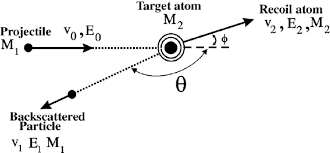
\includegraphics{RBS.png}
	\caption{A diagram of Rutherford Backscattering}
	\label{fig:RBS}
\end{figure}
\subsection{Cross Section}
If the cross section of the RBS event is low, then we will not see any scattering occur, even at very low scattering angles.
The probability of the scattering event is given by the cross section $\sigma$ (area of target atom), number of scattering atoms $N$ per overall area $A$:
$$ P = \frac{N}{A}\sigma$$
For the number of scattering events per unit time, $I$ in terms of this probability and the incident beam current $I_0$ as $I = I_0 P \rightarrow = \frac{I_0 N}{A} \sigma$.
If we assume Rutherford scattering, we just have Coulomb scattering, i.e., there is no screened potential that we need to account, since we are interacting directly with the target nuclei.
If $M_t << M_p$, then the \textit{differential cross section} can be written as:
\begin{equation}
	\frac{d\sigma}{d\Omega} = \left( \frac{Z_pZ_t e^2}{16\pi\epsilon_0 E}\right)^2 \frac{1}{\sin^4 \left(\theta / 2 \right)}
\end{equation}
This is the singularity for when the cross section is zero implies that the projectile never comes close to the target, but in this case it also never penetrates the electron cloud surrounding the nucleus either.
The pure Coulomb formula for the scattering cross section must be correct for this screening effect, which means it becomes more important as the energy of the projectile decreases.
It is important to note the following proportionality of the differential cross section.
$\propto (Z_p Z_t)^2 $ means that the projectile with higher charge ( or atomic mass) are advantageous, i.e., Helium is then better than just Hydrogen.
$\propto E^{-2}$ means that an increase in $E$ leads to a decrease in yield.
This is not good because we want to measure the most possible number of backscattered ions.
$\propto 1 / \sin^4 \theta / 2$ means that a decrease of yield with increasing $\theta$.
An example for a layered example of TiO$_2$ and Sapphire (Al$_2$O$_3$), and using literature values of $\kappa _{Ti} = 0.7171$, $\kappa_O = 0.3626$, $\kappa_{Al} = 0.5526$.
Fitting the values, we can determine the thickness of the layer of titanium oxide to be about $720$nm.


\section{PIXE}
Instead of interacting with the nucleus of the target atom, \textbf{P}article \textbf{I}nduced \textbf{X}-Ray \textbf{E}missions,  or \textbf{PIXE}, is a characteristic of scattering in which the ion beam interacts with the atomic shell of the target atom.
For interactions with the nuclei, this \textbf{P}article \textbf{I}nduced \textbf{G}amma-Ray \textbf{E}missions, or \textbf{PIGE}.
A process that occurs simultaneously with PIXE is the secondary electron emission which one can also analyze.
At higher electronic orbitals we have a phenomena called ion luminescence, where because of the higher orbital interaction, photons with wavelengths in the visible light range are emitted.
PIXE is used by geologists, archaeologists, and even art historians since it is a non-destructive elemental analysis technique that can help answer questions of provenance, dating, and authenticity.
Three types of spectra can be collected form a PIXE experiment: X-ray, Rutherford backscattering, and Proton transmission spectrum.
For X-ray emission, quantum theory states that orbiting electrons must occupy discrete energy levels in order to be stable.
If we bombard a sample with high enough energy ions (MeV protons), then the inner shells of the target atom will become ionized.
Outer shell electrons drop down to replace inner shell vacancies, however only the certain transitions are allowed, thus X-rays of these characteristic energy of the element are emitted.
A detector is used to record and measure these X-rays.
Only elements heavier than fluorine can be detected.
For a quantitative approach, the characteristic equation for the yield (measured inside the detector) is given in the lecture is written as follows:
\begin{equation}
	Y_X (Z) = \frac{N_A \omega_Z b_X \epsilon N_I c_Z}{A_Z} \int_{E_0}^{E_t} \frac{\sigma_Z (E) T_Z(E)}{S(E)} dE
\end{equation}
where $N_A $ is Avogadro number,
$\omega_Z$ the fluorescence yield of transition of element Z,
$b_X$ is the branching ratio, i.e.,  relative Intensity of line in the series of lines,
$\epsilon$ is the efficiency of the detector,
$N_I$ the number of incident particles ,
$c_Z$ the mass concentrations of emitting element Z,
$A_Z$ the mass number of emitting element Z,
$E_0$ the initial energy of incident particles,
$E_t$ the energy of ions after transmission through the sample or $E_{tmax} = 0$,
$Z(E)$ the ionization cross section,
$S(E)$ the stopping of the sample,
$T_Z(E)$ the transmission factor of the x-ray line X.

\section{Ion Beam Induced Charge}
Every charged particle (10 eV) deposits energy into a solid via Coulomb interaction.
This will create electron holes / pairs in the solid that we can use, for example quality checks in semiconductor devices.
Let's assume we have a solid and we are hitting it with an ion beam in the range of MeV.
There will be penetration into the solid and during the Coulomb interaction, we will produce energy transfer into the electrons of the solids, and thus holes/pairs in the neighbourhood of the ion path.
We will thus have a cone shaped plasma inside the solid created by depositing energies and thus producing electrons and holes (positively charged since electrons have left).
If we are using MeV, then we have a depth within the sample of a few $\mu$m and the cone of plasma will be much smaller in radius than the range.
\subsection{Klein Model}
The model developed by Klein, states that the amount of energy needed to create an electron-hole-pairs (EHP), is largely independent of the energy of the sample and type of ionizing radiation from your ion beam.
For example, for silicon we have an energy of 3.26 eV at 300k, and we use an ion at 1 MeV, we will produce lots of EHP, and create a large amount of free charge carriers.
The consequence of the Klein model is that if we use MeV ions on a single ion track, we can produce measurable signals found in pulse height spectrum (PHS).
This is done fore example, by irradiating a sample (an silicon integrated circuit) with ions in MeV region and connect the sample with a charge counter, then we get pulses in the form of a historgram, of events where we produce EHP.
The average of this histogram is then proportional to the change in the electrode.Can help in finding the quality or efficiency of a semiconductor device.

\subsection{Gunn Theorem}
\begin{wrapfigure}{r}{0.5\textwidth}
	\centering
	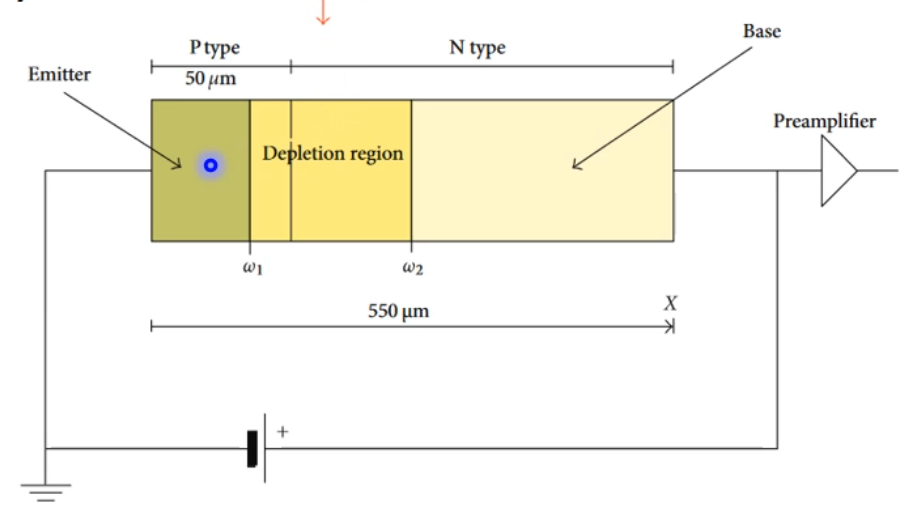
\includegraphics[scale=0.25]{gunndevice}
	\caption{A typical semiconductor diode used to demonstrate Gunn Theorem. A 5 MeV proton beam hits the sample normal to the top of the device. The device is connected to some voltage to suck away the free charge carriers produced by the proton beam. Some electronics like the preamplifier can be used to count the pulses and thus produce a histogram spectrum. }
	\label{fig:semidevice}
\end{wrapfigure}
Developed in 1964, Gunn Theorem, observed by J.B. Gunn in materials with energy band structures, and is a quantitative approach to the Klein model.
We can calculate the expected current at a position within a device given an impact of an ion beam using the equation below.
An example of such a semiconductor device is given in Figure~\ref{fig:semidevice}.
$$ I_i = -q \vec{v} \frac{\partial \vec{E}}{\partial V_i} $$
We have a charged particle, for example a proton beam, $q$ in the above equation would be one, that is traveling wih some velocity $\vec{v}$.
We have then the electric field $\vec{E}$ derivative with respect to the bias voltage applied to the sample.
If we have lots of devices, with various connections, then we could calculate this current for the various junctions, which is indicated with the $i$ subscript.
This partial derivative, is Gunn's weighting field.
Now, we could also calculated the charge produced overtime with this current, $Q_i(t)$.
$$Q_i(t) = \int_0^t I_i(t^{\prime}) dt^{\prime} = -q \int_{r_l}^{r_F} \frac{\partial \vec{E}}{\partial V_i} d\vec{l} = q \left[ \frac{\partial \psi}{\partial V_i} |_{r_F} - \frac{\partial \psi}{\partial V_i} |_{r_l} \right]$$
This is just the integration of the current over time, since charge is current over time.
We could then transform the integral to integrate over the length of the sample using Gauss theorem, since the potential of the electric field has the relation $\nabla \psi = -E$.
In the end we are able to get a relationship between the incident beam and the charge (or current) within the diode.
In the continous case, we have
$$ Q_i(t) = -q \int_0^t dt^{\prime} \int_{\Omega}  d^3 r \left[ x(\vec{r},t) \vec{v}_x (\vec{r}) \frac{\partial\vec{E}}{\partial V_i} \right]$$
\newpage
\begin{wrapfigure}{l}{0.5\textwidth}
	\centering
	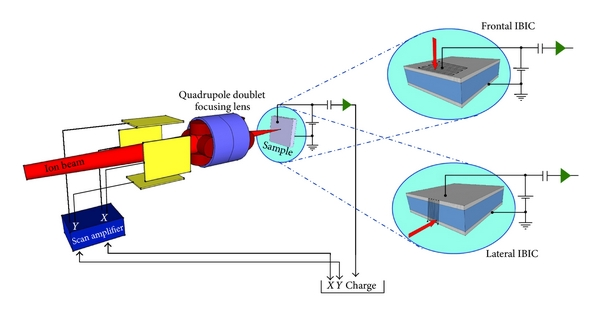
\includegraphics[scale=1.5]{ibic.jpg}
	\caption{Scheme of the IBIC setup. A MeV ion beam from an accelerator is focused by a quadrupole lens system and scanned over the sample surface using two sets of magnetic or electrostatic plates. The insets on the right sides show the two irradiation geometries: from the top (frontal IBIC) and from the side (lateral IBIC) of the device under analysis. Each incident ion generates a measurable charge pulse, which is amplified and processed by a standard charge sensitive electronic chain. The data acquisition system acquires and stores every event along with the coordinates of the ion. \cite{5}}
	\label{fig:ibicmic}
\end{wrapfigure}
These methods can be used for microscopy, which can be seen in Figure~\ref{fig:ibicmic}.
If we scan the beam over the sample, we can get an image if the charge creation within the sample from the incident beam creating charges.
The histogram will then be the amount of charge one gets at a certain position, based on the scanning of the beam.
This will give us insight into the quality of the device, and is often used to check the quality of integrated circuits.
It is also possible to use this technique for the detection of single ions, which is especially useful for quantum computing.
We know that quantum computing needs to be scalable, so if we are to use ion implantation, we must be sure that we are inserting single ions correctly.

\section{Summary}
There are of course many other forms of scattering, some of which are not covered in detail here but are of note.
There is Elastic Recoil detection (ERD), which is used to obtain elemental concentration depth profiles in thin films.
Nuclear reaction analysis (NRA) is a method of nuclear spectroscopy to determine concentration versus the depth distributions for certain target chemical elements in a solid thin film.
\begin{myitemize}
	\item RBS is based of the elastic scattering of the ion with a target atom (ion-nucleus interaction)
	\item PIXE and PIGE are interactions of the ion with the target electron orbitals, the latter being of higher orbital interactions
	\item IBIC Klein Model, creating EHP is largely independent of sample energy as well as type of ionizing radiation.
	\item The methods of precise ion beams are good for quality assessment, or for implanting ions, but also for detecting single ions that wer previously implanted.
\end{myitemize}

%! Author = adam
%! Date = 28.02.21

\chapter{Ion Beams in Semiconductor Physics}\label{ch:ion-beams-in-semiconductor-physics}
Another application of ion beams is their use in semiconductor physics.
Ion beams play a big role in the production of every day life technologies.
The transistors that sit within your phone or laptop are produced using ion beam implantation techniques.
The basics of this requires a basic understanding of semiconductor physics.
If we want to create integrated circuits, we are normally using silicon.
This is because of the energy band gap, $E_g$, between the conduction band and the valence band in the material.
For silicon, this energy band gap is about 1.12 eV.
Usually we use mono-crystalline silicon, and since it is a semiconductor, we will not have a high amount of charge carriers.
The higher the energy gap, the lower the intrinsic charge carrier density (see Fermi-Dirac statistics).
If we want to produce circuits, we can not use crystalline semiconductors, because there is too low intrinsic charge carrier density.
At room temperature, there is about $10^{10}$ charge carriers per cm$^3$, which is relatively low.
Without doping, the density of states (DOS), we have only little amount of holes in the conduction and valence bands, and is the same size for both.
There are several possibilities to produce higher charge concentrations in a semiconductor.
\section{Implantation}
\begin{wrapfigure}{r}{0.6\textwidth}
	\centering
	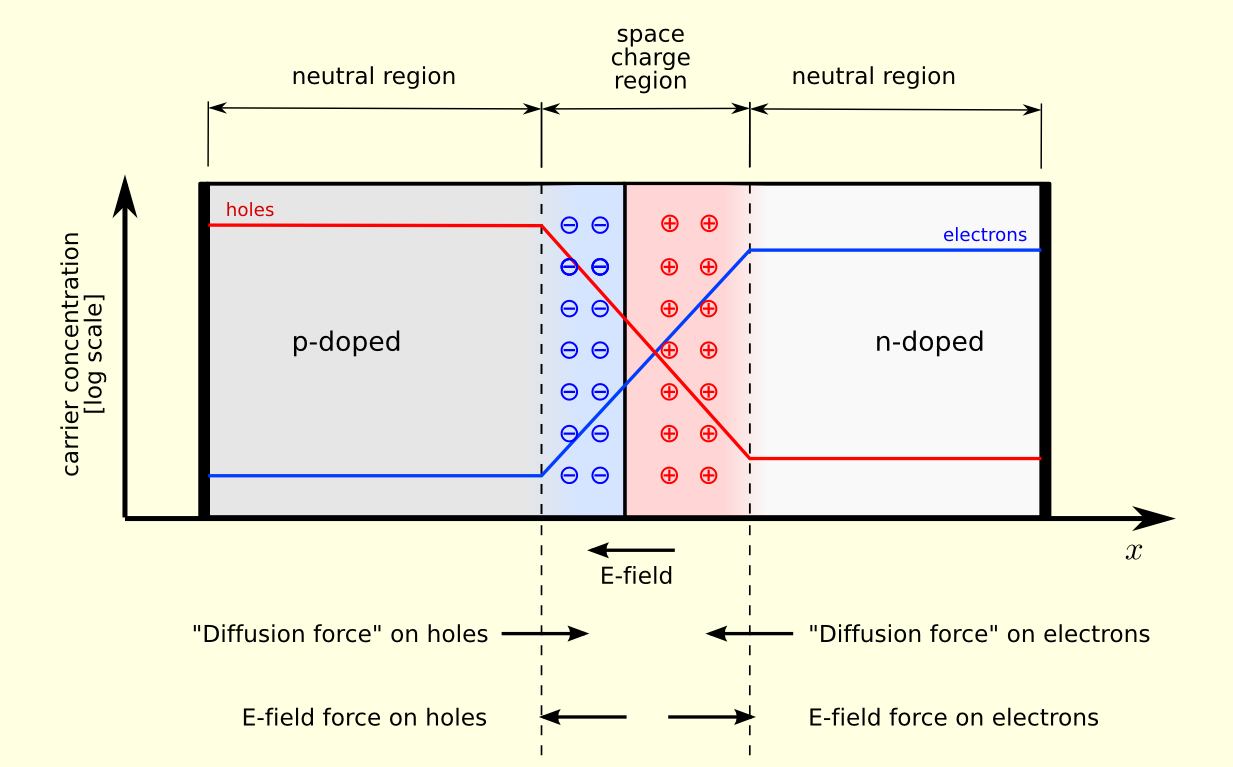
\includegraphics[scale=0.35]{pnjunc.png}
	\caption{A p–n junction in thermal equilibrium with zero-bias voltage applied. Electron and hole concentration are reported with blue and red lines, respectively. Gray regions are charge-neutral. Light-red zone is positively charged. Light-blue zone is negatively charged. The electric field is shown on the bottom, the electrostatic force on electrons and holes and the direction in which the diffusion tends to move electrons and holes.}
	\label{fig:pnjunc}
\end{wrapfigure}
We mentioned that with pure silicon crystals we have low charge carriers, so we could dope the silicon to tune the conductivity of the silicon.
In this process, we add another element other than silicon, for example arsenic, which has one electron more than silicon.
This additional electron can deliver itself to the conduction band, and we have a negative charge carrier, thus this type of silicon would be called \textbf{n-type}.
On the other hand, we could have positive charge carriers implanted, if for example we added boron to the lattice, which has one less electron, and thus one unbounded binding, i.e., we are missing an electron.
This results to a so-called mobile hole, and is almost like an electron with a positive charge, thus the name \textbf{p-type}.
With n-type we have thus much more electrons in the conduction band, because there is an increase in the DOS in the conduction band, and the shifting of the fermi energy towards this conduction band (for non-zero temperature, the fermi energy is replaced with the chemical potential).
One can play around with this kind of doping, an example is something called the PN junction found in Figure \ref{fig:pnjunc}.
We can use ion beam techniques to produce such p-n junctions!
By using ion beams, we can implement these dopants.
At some point there will be a middle point in the junction, in which the range of the n type ion beams and p type ion beams are the same, which you can see in the figure to the right.
So using the knowledge of the range of a particular ion beam in a sample, we can create certain levels in samples using different ion beams with varying energies (leading to different ranges), that can get increasingly sophisticated.
Implantation energies are typically 1keV to 1MeV.
The ion distributions have depths of between 10 nm to 10 $\mu$m.
Doses vary from $10^{12}$ ions per cm$^2$, and voltage adjustments in MOSFETs to 10$^{18}$ ions per cm$^2$ for formation fo buried insulating layers.
Methods of implantation can vary widely depending on the size of the sample.


\section{Annealing}
On the contrary to implantation, we have annealing, which is the process of repairing implant damage, i.e., 'healing' the surface by heating the sample.
Sometimes the process of implantation destroys other sites in the sample, thus necessitating a repair process after the implantation.
Not only does the repair the damage by the ions, but also puts the dopant atoms in substitution sites where they are electrically active.
There are generally two objectives/regimes of different temperature ranges for annealing.
One is the healing, or recrystallization, which is done in temperature ranges of 500--600 C.
The second is the renewing of electrical activity, 600--900 C.
As the lattice becomes repaired, the dopant atoms also fall into place in the lattice, and in the end we have a more or less perfect crystal just with various dopants spread across the lattice sites, adding electrons or holes depending on the doping.
The annealing process depends on the dopant type and dose.
For a given dose, annealing temperature is the temperature at which 90 percent of the implanted ions are activated by a 30-minute annealing in conventional furnace.
For example, boron needs a higher annealing temperature for higher doses.
At lower doses, p-type annealing is similar to n-type.
When the dose is greater than $10^{15}$ cm$^{-2}$, the annealing temperature drops to about 600C.
At doses greater than $6\times 10^{14}$cm$^{-2}$, the silicon surface becomes amorphous, and semiconductor underneath the amorphous layer is a seeding area for recrystallization.
For example, a 100--500 nm amorphous layer can be recrystallized in only a few minutes.
\section{Crystal Generation}
Using Cesium sputtering, we can get negatively charged ions and implant them into a silicon lattice, destroying the crystal order.
There are various regimes about this process, for example, some implanted ions will sputter away intrinsic ions, while in other cases the ions will just be implanted without erosion.
Based on the implantation energy of the ion, we have different sputtering yields, i.e., replacing intrinsic atoms with ions.
We are interested in this to see how different crystals can be created using these techniques.
We could then replace single target atoms with specific ions we want, i.e., building your own specialized lattice, and isotopically enriching layers.
An important result from this is that when combined with annealing, we can decrease spin noise, and increase coherence times (useful for quantum computing).
\section{Summary}
\begin{myitemize}
	\item Using ion beams, we know exactly how deep an ion will penetrate into a sample (range) and thus can construct diodes like p-n junctions
	\item We could also repair these devices using heating (annealing)
	\item we can generate crystals using ion beams, and combine these methods with annealing to get better coherence times and decrease spin noise.
\end{myitemize}


\begin{thebibliography}{9}

\bibitem{1}
Harold Patterson Mahon.
\textit{Design of an electrostatic deflector for the ion beam of the Oregon State College cyclotron}.
Oregon State University, 1954.

\bibitem{2}
Richard Rhodes
\textit{The Making of the Atomic Bomb}
Simon and Schuster, 1986

\bibitem{3}
J. F. Ziegler, J. P. Biersack, and U. Littmark.
\textit{The stopping and range of ions in solids},
The stopping and ranges of ions in matter, vol 1,
Pergamon Press, New York, New York, 1985.

\bibitem{4}
University of Helsinki.
\textit{Notes on Plasma Physics}.
\href{http://beam.helsinki.fi/~knordlun/mdh/rangetext.html}{online}.

\bibitem{5}
Vittone Ettore.
\textit{Semiconductor Characterization by Scanning Ion Beam Induced Charge (IBIC) Microscopy}.
International Scholarly Research Notices, 2013.
\href{https://doi.org/10.1155/2013/637608}{doi}

\bibitem{chen}
Francis F. Chen.
\textit{Introduction to Plasma Physics},
Plenum Publishing, New York, New York, 1977

\end{thebibliography}

\end{document}